%% For normal draft builds (figs not displayed hence fast compile)
%\documentclass[hyperpdf,nobind,draft,oneside]{hepthesis}
%\documentclass[hyperpdf,nobind,draft,twoside]{hepthesis}

%% For short draft builds (breaks citations by necessity)
%\documentclass[hyperpdf,nobind,draft,hidefrontback]{hepthesis}

%% For Cambridge soft-bound version
\documentclass[hyperpdf,bindnopdf]{hepthesis}
%% For Cambridge hard-bound version (must be one-sided)
%\documentclass[hyperpdf,oneside]{hepthesis}

%% Load special font packages here if you wish
\usepackage{lmodern}
\usepackage{mathpazo}
\usepackage{lmodern}
\usepackage{mathpazo}
\usepackage{braket}
\usepackage{siunitx}
\usepackage{acronym}
\usepackage{xspace}
\usepackage{morefloats,subfig,afterpage}
\usepackage{mathrsfs} % script font
\usepackage{verbatim}
\usepackage{tikz}
\usepackage{multirow}
\usepackage[backend=bibtex,url=false]{biblatex}
\usetikzlibrary{external}% activate!
\usepackage{tikz-timing}
\setmainmatterspacing{double}

%%% Useful Commands %%%

\immediate\write18{perl texcount.pl \jobname.tex -1 -sum=1 -merge -out=\jobname.sum}
\newcommand\wordcount{\input{\jobname.sum}}
\addbibresource{Thesis.bib}
\graphicspath{{Figures/Chapter1/}{Figures/Chapter2/}{Figures/Chapter3/}{Figures/Chapter4/}{Figures/}{Figures/Chapter5/}{Figures/Chapter6/}}


\newcommand{\Muquans}[0]{\(\mu\)Quans\xspace}
\newcommand{\sivalue}[2]{\SI[mode=text]{#1}{#2}}
\newcommand{\keff}{{\textbf k_\textnormal{eff}}}
\newcommand{\pow}[2]{\(#1 \times 10^{#2}\)}
\newcommand{\mf}[0]{\(m_\textnormal{F}\)}
\DeclareSIUnit\inch{in}
\DeclareSIUnit\gauss{G}
%% Disables warning about Command terminated with a space
%chktex-file 1


\title{Inertial Navigation using Atom Interferometry}
\author{Jimmy Stammers}

%% Doc-specific PDF metadata
\makeatletter%
\@ifpackageloaded{hyperref}{%
\hypersetup{%
pdftitle = {Inertial Navigation using Atom Interferometry},
pdfsubject = {Jimmy Stammers’ PhD thesis},
pdfkeywords = {atom interferometry, navigation, physics, Rubidium},
pdfauthor = {\textcopyright\ Jimmy Stammers},
colorlinks=false,
linkcolor=black
}}{}

\title{Inertial Navigation using Atom Interferometry}
\author{Jimmy Stammers}

%% Doc-specific PDF metadata
\makeatletter%
\@ifpackageloaded{hyperref}{%
\hypersetup{%
pdftitle = {Inertial Navigation using Atom Interferometry},
pdfsubject = {Jimmy Stammers’ PhD thesis},
pdfkeywords = {atom interferometry, navigation, physics, Rubidium},
pdfauthor = {\textcopyright\ Jimmy Stammers},
colorlinks=false,
linkcolor=black
}}{}
\makeatother

\begin{document}

\begin{frontmatter}
    \titlepage[Department of Physics\\
Centre for Cold Matter]{A thesis submitted to Imperial
  College London for partial
fulfillment of the requirements for the degree of Doctor of Philosophy }
\begin{abstract}
    Matter-wave interferometry has enabled high precision measurements of
    inertial forces such as gravity and the
    Coriolis force. This is facilitated by the long-term stability of
    the physical properties of atoms and lasers. Recent experiments have
    demonstrated the operation of portable, robust sensors using atom
    interferometry. This has potential uses in the context of inertial
    navigation, where conventional devices suffer from long-term
    drifts due to bias instability. Furthermore, determining position
    via dead reckoning requires minimisation of dead time between
    measurements. This thesis presents the development of an atom
    interferometer for measuring horizontal accelerations. In this
    configuration, gravity induces motion across
    the laser wavefront, which constrains the tolerable level of
    wavefront distortions. Effective control of the experiment allows
    the interferometer to be operated at a rate of \sivalue{4}{\Hz}. A cold ensemble of $10^6$ atoms in the same
    internal state is prepared in \sivalue{150}{\ms}. The
    interferometer operates
    using a sequence of three laser pulses separated by
    $T=$ \sivalue{25}{\ms} to achieve sensitivity
    to horizontal accelerations. Combining this with a classical
    accelerometer provides a method of correcting for
    vibration-induced noise, as well as determining the interferometer
    fringe order. After an integration time of \sivalue{70}{\s}, the
    sensitivity to horizontal accelerations is better than
    \sivalue{1e-6}{\m\s\tothe{-2}}. Effects which limit this
    sensitivity are discussed.
 \end{abstract}
\begin{declaration}
  I declare that this thesis is the result of my own work. All sources
  used for this work have been clearly referenced in accordance with
  the departmental requirements.   
        \vspace*{1cm}
        \begin{flushright}
        Jimmy Stammers
        \end{flushright}
        \vfill
  The copyright of this thesis rests with the author and is made
available under a Creative Commons Attribution Non-Commercial No
Derivatives licence. Researchers are free to copy, distribute or
transmit the thesis on the condition that they attribute it, that they do
not use it for commercial purposes and that they do not alter,
transform or build upon it. For any reuse or redistribution,
researchers must make clear to others the licence terms of this
work.
\end{declaration}
\begin{acknowledgements}
    There are many people to whom I owe a great deal of thanks. 
\end{acknowledgements}

%\begin{preface}
%    This thesis describes my research on various aspects of\ldots
%\end{preface}

%\begin{frontmatter}
    %   \dedication{For the World}
    %   ...
%\end{frontmatter}

\tableofcontents
\listoffigures
\listoftables
\frontquote{I may not have gone where I intended to go, but I think I
have ended up where I needed to be}{Douglas Adams}

\end{frontmatter}

\begin{mainmatter}
    \chapter{Introduction}\label{chap:intro}
\section{Technology and Quantum Mechanics}
Throughout history, scientific progress has paved
the way towards great technological and societal advances. A
(relatively) modern
example of this is the development of quantum mechanics,
around the start of the 20\textsuperscript{th} century. This led to
vast improvements in the understanding of the physical world at the
microscopic scale. Eventually, the application of quantum theories of
matter and light led
to technological discoveries which have hugely impacted upon
subsequent scientific research, as well as our general lifestyle. These benefits are not always immediately obvious. For
instance, around the time that the laser was
discovered~\cite{Schawlow1958}, it
was believed that a coherent source of light was of little practical
use
outside of spectroscopy. Of course, the widespread use of commercial laser systems in
medicine and telecommunications show that this is not the case.
Another such example is the development of semiconductor electronics, which started with the transistor and has revolutionised
modern life with the plethora of devices seen today. 
\par\noindent
Broadly speaking, these technologies rely on quantum phenomena that
exist within
bulk matter, i.e. macroscopic ensembles of quantum objects. 
These do not exhibit the microscopic quantum phenomena such as
entanglement and interference. They are open systems, which interact strongly with their
environment causing a loss of coherence across the ensemble. For
this reason, there has been a
growth in research that has focused on the control of
individual quantum systems, such as atoms, molecules and photons.
Experimentally, these can be well-isolated from their environment so
that the coherence between quantum states affects the dynamics of the
system. Technologies aimed at controlling quantum systems have
progressed to the point where it is now possible to engineer robust
devices that make use of quantum effects. This is well-known in the
context of quantum computing and quantum cryptography, which offer
many benefits over their classical counterparts. 
\par\noindent
The field of metrology has also shown great increases in measurement
precision using quantum systems. The archetypal example of this is the
atomic clock~\cite{ESSEN1955}, which uses the interference between two internal states
of an atom such as Caesium-13 to
measure their transition frequency. Owing to their frequency
stability, atomic clocks are now used to implicitly define the
second in terms of physical constants and provide a continuous,
precise time scale~\cite{Levine}.

\section{Inertial Navigation}
The ability to measure inertial forces, i.e. accelerations and
rotations, is of
great practical interest. This is strongly motivated by the need for
inertial navigation systems. In general, these make use on on-board
sensors to determine its position using the process of dead reckoning.
The acceleration and rotation are periodically measured and the
position of the object relative to its initial position is determined by
integrating these forces. The accuracy of this method depends upon the intrinsic noise and bias of these devices. These
lead to a position error which grows in time. For instance, the
effects of white noise are discussed in~\cite{Wen2016}. In the context
of this project, the effects of a sensor's stability over time is
discussed more quantitatively using the Allan variance
in~\SectionRef{subsec:allan_variance}.
\par\noindent
Generally, the
position error due to sensor noise can be reduced through statistical
techniques such as Kalman filtering. This produces an un-biased estimate
of the updated position by taking the noise of each sensor into
account. The position error due to a bias must be addressed
separately. A constant acceleration bias, $\epsilon$ leads to a
position error that grows quadratically in time. An initial
calibration of the sensor can remove this bias, but cannot account for
drifts over time. This phenemenon, often termed bias instability, is
the result of effects such as temperature variations and mechanical
strains. This leads to a characteristic time beyond which the
measurement uncertainty is not reduced by averaging the signal. This
problem can be alleviated by regularly correcting for the position
error using an external positioning system, such as \ac{gnss}, and
re-calibrating the sensors.
\subsection{Improving Long-Term Stability with Atom Interferometry}
Experiments over the past few decades have highlighted the prospect of
using cold atoms for precise inertial sensing. Once cooled to the
\sivalue{}{\mu\K} regime, the thermal velocity of an atomic ensemble
is small enough that they can be controlled for durations up to the order
of seconds. Early experiments by Kasevich and Chu into matter-wave
interferometry of Sodium atoms demonstrated the 
It has been suggested that the problem of bias instability can be
overcome by using cold atoms to measure inertial forces.  
For instance, there exist commerically available \ac{mems} devices
which have a noise level of $\sim \sivalue{5}{\mu\g}$ in the
0-\sivalue{100}{\Hertz} bandwidth. Since the noise between successive
measurements is uncorrelated, the position error  After many successive measurem  
\section{Thesis Overview}
This thesis is structured as follows. A theoretical introduction to
matter-wave interferometry and the relevant atomic structure of
\ac{rb87} is presented in~\ChapterRef{chap:theory}. This is followed
by a description of the software that was developed to control the experiment and
acquire data in~\ChapterRef{chap:compinterface}. The subsequent chapters
focus on various experimental aspects of the project. The preliminary
cooling and trapping of \ac{rb87} is presented
in~\ChapterRef{chap:mot}. The techniques used to cool the atoms
further and prepare an ensemble in the same internal state are
explained in~\ChapterRef{chap:atom_prep}. This is followed by the
design and characterisation of an in-vacuum optical system for driving
Raman transitions in~\ChapterRef{chap:raman_optics}. Finally, a
characterisation of acceleration-sensitive interference is given
in~\ChapterRef{chap:atom_int}.




    \chapter{Theory}\label{chap:theory}
\section{Chapter Overview}\label{sec:theory_overview}
This chapter presents a theoretical discussion of the interaction
between light and matter that forms the basis of atom interferometry.
It begins with a review of the theory of matter-wave interference and
its application to measuring inertial forces such as accelerations
in~\SectionRef{sec:theory_atomint}. This is followed by a derivation of
the equations of motion for a Raman transition in a simplified
three-level atom
in~\SectionRef{sec:theory_raman}. Finally, this chapter concludes with
a discussion of the atomic structure of \ac{rb87}, focusing on the
aspects relevant to the previously mentioned phenomena.
\par\noindent
This chapter assumes some prior understanding of light-matter
interactions on the part of the reader. A comprehensive description of
the semi-classical approximation to atom-light interactions can be
found in~\cite{Grynberg2011}. Theories on laser cooling and magneto-optical
trapping are of interest to some experimental aspects of these thesis.
Details of these can be found in~\cite{Metcalf2003}. For an exact derivation of
the two-level approximation to the Raman transition, the reader is referred
to~\cite{Wu1996}.  
\section{Light-Pulse Matter-Wave Interference}\label{sec:theory_atomint}
A cornerstone of quantum mechanics is the wave-like evolution of
quantum states as described by the Schr\"odinger equation. As a
consequence of this, it is possible to create superpositions of states
that evolve coherently. Furthermore, these states can interfere with
each other if their wavefunctions overlap. The interference pattern,
which depends on the difference in phase between the two paths.
\par\noindent
In this section, the theory of matter-wave interference using pulses
of laser light is presented. It begins with a description of the
$\pi/2-\pi-\pi/2$ pulse sequence that forms an analogue of the
Mach-Zehnder interferometer in~\SectionRef{subsec:theory_mz}. This is
followed by a derivation of the interferometer phase in~\SectionRef{subsec:theory_path}. In
particular, it is shown that this depends upon the
acceleration of the atom during the interferometer. 

\subsection{The Mach-Zehnder Scheme}\label{subsec:theory_mz}
One method for realising matter-wave interference is the
Ramsey-Bord\'e interferometer. This requires an ensemble
of atoms that can be driven between two states using an interaction
with a laser field. The absorption and stimulated emission of photons
exchanges momentum between the atom and the light such that the state
of the atom is defined as a product of its internal states and
momentum eigenstates, labelled as $\ket{1,\textbf{p}}$ and
$\ket{2,\textbf{p} + \hbar \textbf{k}}$. When compared with
conventional optical interferometry, it is the light which alters the
trajectory of the matter, rather than the other way around. Indeed,
laser pulses with pulse areas of $\pi/2$ and $\pi$ are analogous to
beam-splitters and mirrors in optical systems.  
\par\noindent
A three pulse interferometer is the simplest configuration for which
the two trajectories can overlap after separation. Schematically, this
is shown in~\FigureRef{fig:interferometer}. An atom in
$\ket{1,\textbf{p}}$ is driven into a superposition of two states
using a $\pi/2$ pulse. The wavepacket in $\ket{2,\textbf{p} + \hbar
\textbf{k}}$ has a different momentum, so the two become
spatially separated. After a time $T$, a $\pi$ pulse inverts the state
along each path, so that after another duration of $T$ the two
wavepackets overlap. These are recombined by a final $\pi/2$ pulse.
The interference between the two states is manifested in their
population, which depends on the phase difference between the two
paths. This phase difference $\Delta \Phi$ is expressed as follows
\begin{equation}
  \label{eq:phase_difference}
  \Delta \Phi = \Delta \Phi_\textnormal{prop} +\Delta
  \Phi_\textnormal{int}+\Delta \Phi_\textnormal{laser}
\end{equation}
where $\Delta \Phi_\textnormal{prop}$ is the phase difference due to
propagation along each path, $\Delta \Phi_\textnormal{int}$ is the
phase difference due to evolution of the internal state and $\Delta
\Phi_\textnormal{laser}$ is the phase difference caused by
interactions with the laser field.   
\begin{figure}[htpb]
  \centering
  \resizebox{0.8\textwidth}{!}{\input{interferometer.pdf_tex}}
  \caption[Mach-Zehnder atom interferometer configuration.]{Mach-Zehnder atom interferometer configuration. A sequence
  of laser pulses are used to drive an atom into a superposition of
two states. When the two paths overlap at the final $\pi/2$ pulse,
they interfere with each other. The final occupation probability is
proportional to the phase difference between the two paths.}
  \label{fig:interferometer}
\end{figure}

\subsection{Phase Shift Contributions}\label{subsec:theory_path}
\subsubsection{Propagation Phase}
The propagation phase can be evaluated using the path integral
approach to quantum mechanics. The trajectory of
a quantum state is obtained by integrating over all possible paths.
The total amplitude for arriving at position $x_b$ at $t_b$, starting
from $x_a$ at $t_a$ is given by the following propagator
\begin{equation}
  K(t_b,x_b,t_a,x_a) = \int_{x_a}^{x_b} e^{i S/\hbar} \mathrm{d}x(t)  
\end{equation}
where $x_b \equiv x(t_b)$ and similarly for $x_a$. The action $S$
along a path is
defined using the Lagrangian of the system
\begin{equation}
  S = \int_{t_a}^{t_b} L(x,\dot{x})\; \mathrm{d}t
  \label{eq:action_def}
\end{equation}
and the classical limit is recovered when the action $S_\textnormal{cl}
\gg
\hbar$. In this case, most paths destructively interfere as their
phases oscillate rapidly. Along the classical path, the action is
minimised. Paths close to this lead to constructive interference, so
the trajectory of the system is well-described using the Euler-Lagrange equations. Under this
condition, it can be shown~\cite{Storey1994} that for a plane wave,
the propagation phase is proportional to the action along the
classical path
\begin{equation}
  \label{eq:prop_phase}
  \Delta \Phi_\textnormal{prop} = \frac{i}{\hbar} S_\textnormal{cl}(t_b,x_b,t_a,x_a)
\end{equation}
\par\noindent
This is indeed the case for an atom interferometer. When considering a
single atom under a constant
acceleration, the Lagrangian is given by
\begin{equation}
  \label{eq:lagrange_acc}
  L = \frac{1}{2}m\dot{x}^2 + m a x
\end{equation}
so that it's position and velocity are given by
\begin{subequations}
\begin{align}
  x(t) &= x_a + v_a (t-t_a) + \frac{1}{2} a (t-t_a)^2 \\
  v(t) &= v_a + a(t-t_a)
\end{align}
\end{subequations}
for initial values of position ($x_a$), velocity ($v_a$) and time
($t_a$).     
Using~\EquationRef{eq:action_def}, the action is given by 
\begin{equation}
  \label{eq:action_classical}
  S(t_b,x_b,t_a,x_a) = \frac{m(x_b-x_a)^2}{2(t_b-t_a)} + \frac{m a
  (x_b+x_a)(t_b-t_a)}{2} -\frac{m a^2 (t_b-t_a)^3}{24} 
\end{equation}
The trajectories along each interferometer path under acceleration is
shown in~\FigureRef{fig:interferometer_accel}. Denoting
$S_\textnormal{ac} \equiv S(T,x_c,0,x_a)$ and likewise for the other
co-ordinates, the difference in the action along the upper and lower paths is 
\begin{align}
  S_\textnormal{ac} + S_\textnormal{cd} -
\left(S_\textnormal{ab}+S_\textnormal{bd}\right) &= -\frac{\text{m}
(x_b-x_c) \left(a T^2- x_a+x_b+x_c-x_d\right)}{T}\nonumber \\
&= -\frac{\text{m}
(x'_b-x'_c) \left((x'_c-x'_a) + (x'_d+-x'_b)\right)}{T}
\label{eq:prop_action}
\end{align}
where the second expression is obtained using $x_b - x_b' = x_c - x_c'
= \frac{1}{2}a T^2$ and $x_d-x_d' = 2 a T^2$. When there is zero
acceleration, the area enclosed by the interferometer forms a
parallelogram and the action along each path is equal. It follows
from~\EquationRef{eq:prop_phase} that $\Delta \Phi_\textnormal{prop} =
0$ when there is a constant acceleration of the atom.
\begin{figure}[htpb]
  \centering
  \resizebox{0.8\textwidth}{!}{\input{interferometer_accel.pdf_tex}}
  \caption[Interferemeter paths under constant
  acceleration]{Interferometer paths under a constant acceleration.
  The dashed lines indicate the trajectories under zero acceleration.}
\label{fig:interferometer_accel}
\end{figure}
\subsubsection{Internal State Evolution}
Between each laser pulse, the atom evolves freely. Therefore, the
phase due to this evolution is given by
\begin{equation}
  \label{eq:internal_evolution}
  \phi^{(j)}(t_a,t_b) = \int_{t_a}^{t_b} i \omega_j t\;\mathrm{d} t
\end{equation}
where $\omega_j$ depends on the state of the atom along that
trajectory. The phase difference due to the internal state evolution
is 
\begin{equation}
  \label{eq:phase_internal}
  \Delta \Phi_\textnormal{int} = \phi^{(2)}(t_1,t_2) +
  \phi^{(1)}(t_2,t_3) - \left(\phi^{(1)}(t_1,t_2) + \phi^{(2)}(t_2,t_3)\right)
\end{equation}
which is zero if the time between successive pulses is the same and
the energy of each state does not vary. The latter case is important
when considering the effects of the ac Stark shift and is addressed
subsequently in~\SectionRef{subsec:light_shift}.

\subsubsection{Laser Phase}
Finally, there is the contribution from the laser phase. During each
transition, the phase of the laser modifies the state of the atom. The
propagator that describes this transition for arbitrary Rabi
frequencies and detuning is derived below,
in~\SectionRef{sec:theory_raman}. For now, it is sufficient to focus
on the ideal case of perfect pulse areas and zero detuning. The laser
interaction modifies the two states as follows
\begin{subequations}
  \begin{align}
    U_\text{L}(\phi) \ket{1} &= e^{-i \phi} \ket{2} \\
    U_\text{L}(\phi) \ket{2} &= e^{i \phi} \ket{1} 
  \end{align}
\end{subequations}
where $\phi = \textbf{k.x} - \omega_\text{L}t + \phi_j$ is the phase
of the light driving the transition. If the time between each pulse is
constant the $\omega_\text{L} t$ term can be omitted, so that the
phase of the atom along each path depends on its position and the
phase of the laser. If the acceleration is along the same axis as the
light's wavevector ($\textbf{k.x} \equiv k x$), the phase along the upper and lower paths are 
\begin{subequations}
  \begin{align}
    \phi_l &= i(k x_b + \phi_2) \\
    \phi_u &= i(k (x_a - x_c + x_d) + \phi_1 - \phi_2 + \phi_3)
  \end{align}
\end{subequations}
Following the same argument used in~\EquationRef{eq:prop_action}, this
can be simplified so that the phase difference due to the laser interaction ($\phi_u -
\phi_l$), and hence the total phase difference, is
\begin{equation}
  \label{eq:phase_interferometer}
  \Delta_\Phi = \Delta \Phi_\textnormal{laser} = \textbf{k.a} T^2 + \phi_1 - 2\phi_2
  + \phi_3
\end{equation}

\section{Raman Transitions in Rubidium-87}\label{sec:theory_raman}
In this section, an analysis of the dynamics of the stimulated Raman transition is
presented. This is modeled as an effective transition between two
ground states $\ket{1}$ and $\ket{2}$. These two states are coupled
via an intermediate state $\ket{i}$ which can be adiabatically
eliminated when the two light fields are sufficiently detuned from
resonance. An explicit derivation of this process can be found
elsewhere
\cite{Moler1992,Weiss1994}. The key results, which aid the discussion
of the performance of the interferometer in subsequent chapters, are
summarised below. Following this, a propagator is derived which
describes the evolution of the atomic state during a Raman transition.
This is used to derive the final state after the interferometer pulse
sequence. Modeling the atomic system in this way makes it possible to consider
the effects of finite pulse duration, detuning and intensity
on the final state. 
\par\noindent
The energy level scheme for a Raman transition is shown
in~\FigureRef{fig:raman_model}. Each ground state is coupled to the
intermediate state $\ket{i}$ by an interaction with an electric field  
$ \textbf{E}_j=
\textbf{E}_{0,j} \cos(\omega_j^l t - \textbf{k}_j.\textbf{x}+
\phi_j)$. The strength of this interaction is defined by the Rabi
frequency\begin{equation}
  \label{eq:rabi_freq}
  \Omega_j = \frac{1}{\hbar}\bra{j} -\textbf{d}.\textbf{E}_{0,j}
  \ket{i} e^{i \phi_j}
\end{equation}
where $\textbf{d}$ is the dipole operator. The frequency of each field is detuned from resonance to
give a two-photon detuning $\Delta$. It is assumed that the
hyperfine splitting $\omega_\text{hfs}$ is much larger than this, so
that each field only drives transitions from one of the ground states. 
%The total electric field is described by the superposition $\textbf{E}_1 + \textbf{E}_2$. 
When $\Delta$ is sufficiently larger than the natural transition
linewidth, the population of the intermediate state remains constant
and can be adiabatically eliminated. The
interference of the two fields means that the transition can be
represented by an interaction with an effective field with the
following parameters
\begin{subequations}
  \begin{align}
    \omega_\textnormal{eff} &= \omega^l_1 - \omega^2_l \\
    \phi_\textnormal{eff} &= \phi_1 -\phi_2 \\
    \keff &= \textbf{k}_1 - \textbf{k}_2 \\
          &\approx 2\textbf{k}_1\;
    \text{(when counter-propagating)} \nonumber 
  \end{align}
\end{subequations}
The resonance condition for the Raman transition is given by 
\begin{equation}
  \delta = \omega_\textnormal{eff} - \left[\omega_\textnormal{hfs} + \keff .
\textbf{v} + \frac{\hbar |\keff|^2}{2m}\right]
  \label{eq:raman_detuning}
\end{equation}
\begin{figure}[htpb]
  \centering
  \fontsize{16pt}{16pt}
  \resizebox{0.4\textwidth}{!}{\input{raman_model.pdf_tex}}
  \caption[Schematic diagram of a raman transition.]{Schematic diagram of a raman transition. Two states,
  $\ket{1}$ and $\ket{2}$, are coupled to each other via transitions
  to an
intermediate state $\ket{i}$. When the frequencies of the light
fields are
far-detuned from resonance,
then $\ket{i}$ can be adiabatically eliminated, resulting in an
effective two-level system.}
  \label{fig:raman_model}
\end{figure}
\subsection{State Propagation}
To describe the dynamics of the Raman transition, it is convenient to
express the system in the interaction picture. This allows the
Hamiltonian to be represented in a time-independent form. An analytic
solution to the equations of motion can then be obtained, which
describes the evolution of the atomic state during a Raman transition. After adiabatically
eliminating the intermediate state~\cite{Weiss1994}, the state of the
atom in a rotating frame is given by
\begin{equation}
  \label{eq:state_raman}
  \ket{\psi} = c_1 e^{-i \omega_1 t}\ket{1} + c_2 e^{-i (\omega_2 +
  \delta) t} \ket{2}
\end{equation}
The Hamiltonian can be simplified by making the rotating wave
approximation, which neglects the rapidly oscillating terms. After
this, the Schr\"odinger equation becomes
\begin{equation}
  \label{eq:raman_eom}
  i \begin{pmatrix} \dot{c}_1 \\ \dot{c}_2 \end{pmatrix} =
  \frac{1}{2} \begin{pmatrix}
    -\Omega_1^\textnormal{ac} & \Omega_\textnormal{eff} \\
    \Omega_\textnormal{eff}^*&  -2 \delta - \Omega_2^\textnormal{ac}  \\
    \end{pmatrix} \begin{pmatrix} c_1 \\ c_2\end{pmatrix}
\end{equation}
Where in terms of the single-photon Rabi frequencies $\Omega_1$ and
$\Omega_2$, the ac Stark shifts $\Omega_j^\textnormal{ac}$ and
effective Rabi frequency $\Omega_\textnormal{eff}$ are given by 
\begin{subequations}
\begin{align}
  \Omega_j^\textnormal{ac} &= -\frac{|\Omega_j|^2}{2 \Delta
  }\label{eq:raman_ac_stark}\\
  \Omega_\textnormal{eff}&=\frac{e^{i\phi_\textnormal{eff}} |\Omega_1|
    |\Omega_2|}{2 \Delta }\label{eq:raman_rabi} 
\end{align}
\end{subequations}
Under an appropriate choice of intensities and two-photon detuning, it
is possible to cancel the differential ac Stark shift
$\Omega_1^\textnormal{ac} -\Omega_2^\textnormal{ac}$ (see
\SectionRef{subsec:light_shift} for further details on this).
Therefore, they can be omitted from~\EquationRef{eq:raman_eom} so that
after solving the Schr\"odinger equation, the coefficients $c_1,c_2$
evolve according to 
\begin{equation}
  \label{eq:schrodinger_prop}
  \begin{pmatrix} c_1(t) \\ c_2(t)\end{pmatrix} = U \begin{pmatrix}
c_1(0) \\ c_2(0)\end{pmatrix}
\end{equation}
where the propagator $U$ is
\begin{equation}
  U = e^{\frac{1}{2}i\delta t } \begin{pmatrix} 
  \cos \left(\frac{ \Omega' t}{2}\right)-i\frac{\delta}{\Omega'}\sin
  \left(\frac{\Omega' t}{2}\right) & 
 -i e^{i \phi_\textnormal{eff}} \frac{
 \Omega_\textnormal{eff}}{\Omega'} \sin \left(\frac{\Omega'
 t}{2}\right) \\ 
  -i e^{-i \phi_\textnormal{eff}} \frac{
  \Omega_\textnormal{eff}}{\Omega'} \sin \left(\frac{\Omega'
t}{2}\right)& \cos \left(\frac{ \Omega' t}{2}\right)+i\frac{
\delta  }{\Omega'}\sin \left(\frac{ \Omega' t}{2}\right) \\
\end{pmatrix}
\label{eq:propagator_first}
\end{equation}
and $\Omega' = \sqrt{\delta^2 + \Omega_\textnormal{eff}^2}$ is the
generalised Rabi frequency. After transforming back into the
stationary frame, \EquationRef{eq:propagator_first} becomes
\begin{equation}
U =  \begin{pmatrix} 
  e^{\frac{i(\omega_\textnormal{eff}-\delta_R)t}{2}  }\left(\cos \left(\frac{ \Omega' t}{2}\right)-i\frac{\delta}{\Omega'}\sin
  \left(\frac{\Omega' t}{2}\right)\right) & 
 -i e^{\frac{i(\omega_\textnormal{eff}-\delta_R)t}{2}  }e^{i \phi_\textnormal{eff}} \frac{
 \Omega_\textnormal{eff}}{\Omega'} \sin \left(\frac{\Omega'
 t}{2}\right) \\ 
  -i e^{\frac{-i(\omega_\textnormal{eff}-\delta_R)t}{2}  }e^{-i \phi_\textnormal{eff}} \frac{
  \Omega_\textnormal{eff}}{\Omega'} \sin \left(\frac{\Omega'
  t}{2}\right)& e^{-\frac{i(\omega_\textnormal{eff}-\delta_R)t}{2}  }\left(\cos \left(\frac{ \Omega' t}{2}\right)+i\frac{
\delta  }{\Omega'}\sin \left(\frac{ \Omega' t}{2}\right)\right) \\
\end{pmatrix}
\label{eq:propagator_stationary}
\end{equation}  
where $\delta_R = \keff.\textbf{v} + \hbar |\keff|^2/2m$ is the Raman
detuning from
\EquationRef{eq:raman_detuning}.
\subsection{Application to a Sequence of Raman Pulses}
Now, this propagator can be used to determine the state of the atom
after a sequence of Raman pulses. The propagator was derived using an
initial state at $t=0$. This can be generalised to an arbitrary time
by replacing $t\rightarrow t-t_0$ and $\phi_\textnormal{eff} \rightarrow \phi_\textnormal{eff} +
\omega_\textnormal{eff} t_0$. Between successive Raman pulses, there is a period of
free evolution for a time $T$. During this, the state evolves
according to
\begin{equation}
  \label{eq:free_evolution}
  F(T) = \begin{pmatrix} e^{-i \frac{\omega_\textnormal{hfs} T}{2}} &0 \\
  0 & e^{i \frac{\omega_\textnormal{hfs} T}{2}}\end{pmatrix}
\end{equation}
Treating the Rabi frequency, phase, detuning and pulse duration as free
parameters denoted by an index $j=1,2,3$, the state after three arbitrary pulses separated in time
is given by
\begin{equation}
  \label{eq:general_state}
  \ket{\psi} = U(\Omega_3,\phi_3,\delta_3,\tau_3) F(T_2)
  U(\Omega_2,\phi_2,\delta_3,\tau_2) F(T_1)
  U(\Omega_1,\phi_1,\delta_1,\tau_1)
  \ket{\psi_0}
\end{equation}
for an initial state $\ket{\psi_0}$. This expression is valid for
arbitrary pulses and is useful when considering a
distribution of intensities and Doppler detunings across an atomic
ensemble. For instance, the occupation probability for $\ket{2}$ is
given by 
\begin{equation}
  \label{eq:occ_prob}
  P_{\ket{2}} = |\braket{2|\psi}|^2
\end{equation}
It is also useful to define the fringe contrast -- the difference
between the maximum and minimum of $P_{\ket{2}}$
\begin{equation}
  \label{eq:fringe_contrast}
  c = \max_{\Delta \Phi} P_{\ket{2}} -  \min_{\Delta \Phi} P_{\ket{2}} 
\end{equation}
which ranges between 0 and 1. This fringe contrast implicitly depends
on the pulse area and detuning of each pulse. In the case of perfect pulse areas and zero
detuning with the initial state $\ket{\psi_0} =
\ket{1}$, \EquationRef{eq:occ_prob} yields the following
\begin{align}
  \label{eq:state_simp}
  P'_{\ket{2}} &= \sin \left(\frac{1}{2} (\phi_1-2
  \phi_2+\phi_3)\right)^2 \nonumber \\
  &= \sin\left(\frac{\Delta \Phi}{2}\right)
\end{align}
Where $\Delta \Phi$, defined
in~\EquationRef{eq:phase_interferometer}, is recovered by substituting 
$\phi_j \rightarrow \phi_j^{(l)} + \textbf{k.x}$ and using the
position of the centre-of-mass at each pulse for $\textbf{x}$.
%In order to observe interference between two atomic states, it is
%essential that they remain coherent over the required timescale. The
%most suitable choice of states for this are the $\ket{F=1,m_F=0}$ and
%$\ket{F=2,m_F=0}$ hyperfine ground states. Neither of these states
%will spontaneously decay and their energy has only a second-order
%dependence on magnetic fields. However, the transition frequency
%$\omega_\text{hfs} \approx 2\pi \times$ \sivalue{6.835}{\GHz} is
%stimulated using microwave radiation, so each photon imparts little
%momentum to the atom. Since the sensitivity of an atom interferometer to
%inertial forces is proportional to the momentum transferred, this can
%be increased by stimulating Raman transitions using light at optical
%frequencies. In this case, an atom will absorb a photon from one light
%field and emit into the other. If the two fields are
%counter-propagating, this has the effect 
\subsection{Extending to a Real Atomic System}

In a real atomic system, there are many intermediate states which
couple to the two ground states. This theory can be extended to
consider the additional intermediate states using their individual
Rabi frequencies. In this case, the effective Rabi frequency is given
by the following sum
\begin{equation}
  \label{eq:rabi_raman_sum}
  \Omega_\textnormal{eff} = e^{i \phi_\textnormal{eff}}  \sum_k
\frac{|\Omega_{1k}| |\Omega_{2k}|}{2\Delta_k}
\end{equation}
where the index $k$ labels the intermediate states which couple to
both $\ket{1}$ and $\ket{2}$. A similar expression can be obtained for
the ac Stark shift terms. The effective Rabi frequency in \EquationRef{eq:rabi_raman_sum} implicitly
depends on the polarisation of the light. The individual Rabi
frequencies $\Omega_{jk}$ are calculated using the Clebsch-Gordan
coefficients that describe the coupling of angular momentum states.
Further detail on calculating transition matrix elements of tensor
operators can be found in~\cite{Brink1968}. 
%\par\noindent
%A Raman transition is a two-photon process whereby the state of an
%atom evolves by interacting with two laser fields. This can occur in
%an atomic system with two states $\ket{1}$ and $\ket{2}$ that are both coupled to an
%intermediate state $\ket{i}$ via electric dipole transitions. The eigenstates
%$\ket{j,\textbf{p}_j}$ are products of the internal state $\ket{j}$ and a momentum
%eigenstate $\ket{\textbf{p}_j} = e^{i
%\frac{\textbf{p}_j.\textbf{x}}{\hbar}}$. In general,
%the state of the atom is a superposition of these eigenstates
%\begin{equation}
%  \ket{\psi} = c_1\ket{1,\textbf{p}_1} + c_2
%  \ket{2,\textbf{p}_2} + c_i \ket{i,\textbf{p}_i}
%  \label{eq:raman_state}
%\end{equation}
%and the Hamiltonian that describes the evolution of this system is
%\begin{equation}
%  H = H_0 + H_I
%  \label{eq:raman_hamiltonian}
%\end{equation}
%where $H_0$ is the free Hamiltonian
%\begin{equation}
%  H_0 = \hbar \begin{pmatrix}
%    \omega_1 + \frac{p_1^2}{2m\hbar}& 0 & 0 \\
%    0 & \omega_2+ \frac{p_2^2}{2m\hbar} & 0 \\
%    0 & 0 & \omega_i+ \frac{p_i^2}{2m\hbar}
%  \end{pmatrix}
%  \label{eq:free_hamiltonian}
%\end{equation}
%and $H_I$ is the interaction Hamiltonian which describes the
%interaction between the atom and the light. Writing the
%electric fields of the respective lasers as $ \textbf{E}_j=
%\textbf{E}_{0,j} \cos(\omega_j^l t - \textbf{k}_j.\textbf{x}+
%\phi_j)$ for $j=1,2$, the interaction Hamiltonian depends upon
%their superposition $\textbf{E}_1 + \textbf{E}_2$. Assuming that the
%energy difference of $\ket{1}$ and $\ket{2}$ is much greater than the
%transition linewidth, each field stimulates transitions from just one of the lower states. In this case, $H_I$ is  
%\begin{equation}
%  \label{eq:interaction_hamiltonian}
%  H_I = \frac{\hbar}{2} \begin{pmatrix}
%    0 & 0 & \Omega_1e^{-i (\omega_1^l t- \textbf{k}_1.\textbf{x}+\phi_1)} \\
%    0 & 0 &\Omega_2 e^{-i (\omega_2^l t- \textbf{k}_2.\textbf{x}+\phi_2)} \\
%    \Omega^*_1 e^{i (\omega_1^l t - \textbf{k}_1.\textbf{x}+ \phi_1)} & \Omega_2^* e^{i
%    (\omega_2^l t - \textbf{k}_2.\textbf{x}+ \phi_2)}& 0
%  \end{pmatrix} + c.c. 
%\end{equation}
%where $\Omega_j$ is the Rabi frequency
%\begin{equation}
%  \label{eq:rabi_freq}
%  \Omega_j = \bra{j} -\textbf{d}.\textbf{E}_{0,j} \ket{i}
%\end{equation}
%and $\textbf{d}$ is the electric dipole operator. 
%In the interaction picture, the state of the atom is given by
%\begin{equation}
%  \ket{\psi(t)} = c_1 e^{-\gamma_1 t} \ket{1, \textbf{p}_1} +c_2 e^{-i
%  \gamma_2 t} \ket{2, \textbf{p}_2} +c_i e^{-i \gamma_i t} \ket{i, \textbf{p}_i} 
%  \label{eq:raman_state_time}
%\end{equation}
%where $\gamma_i \equiv \omega_i + p_i^2/2m\hbar$. The interaction
%Hamiltonian becomes
%\begin{align}
%  \label{eq:hamiltonian_interaction}
%  H_{I,I} &= e^{i H_0 t/\hbar} H_I e^{-i H_0 t/\hbar} \nonumber \\
% &=  \frac{\hbar}{2} \begin{pmatrix}
%  0 & 0 &e^{i \gamma_{1i} t} \Omega_1e^{-i (\omega_1^l t- \textbf{k}_1.\textbf{x}+\phi_1)} \\
%    0 & 0 &e^{i \gamma_{2i} t}\Omega_2 e^{-i (\omega_2^l t- \textbf{k}_2.\textbf{x}+\phi_2)} \\
%    e^{-i \gamma_{1i} t}\Omega^*_1 e^{i (\omega_1^l t -
%      \textbf{k}_1.\textbf{x}+ \phi_1)} & e^{-i \gamma_{2i} t}\Omega_2^* e^{i
%    (\omega_2^l t - \textbf{k}_2.\textbf{x}+ \phi_2)}& 0
%  \end{pmatrix} + c.c.
%\end{align}
%where $\gamma_{ji} \equiv \gamma_j - \gamma_i$. The terms oscillating
%at a fast frequency (implicitly defined as $c.c.$) can now be
%neglected using the rotating wave approximation as over the timescale
%of the interaction, their contribution will average to zero. 
%\begin{equation}
%  \ket{\psi(t)} = c_1(0) e^{-i \omega_1 t} \ket{1} +c_2(0) e^{-i \omega_2 t} \ket{2} +c_i(0) e^{-i \omega_i t} \ket{i} 
%  \label{eq:raman_state_time}
%\end{equation}this system is described by the following
%hamiltonian
\
\section{Applications to Rubidium-87}
This final section places what has been discussed thus far into the
context of Rubidium-87, the atomic species used in this experiment. It
begins with a presentation of the atomic structure of the D2
transition in~\SectionRef{subsec:theory_atomic}. Transitions between
different hyperfine levels are used throughout this experiment. Most
importantly, these are used for cooling and trapping, as well as driving
Raman transitions. This is followed by an overview of the
techniques used to drive counter-propagating Raman transitions
in~\SectionRef{subsec:theory_rb87_raman}. In
particular, this motivates the choice of polarisation used for the two
Raman beams. Finally, this section concludes with a discussion of the
two interferometer paths in~\SectionRef{sec:theory_double_int}.
\subsection{Atomic Structure}\label{subsec:theory_atomic}
Rubidium-87 has a hyperfine structure that is well-suited for a wide
range of experiments. For instance, the energy splitting in the
$5P^{3/2}$ level is large enough that it can be efficiently laser
cooled using one laser to cool and another to prevent dark state
population build-up. 
\par\noindent
In addition to this, the existence of two hyperfine
levels in its ground state presents suitable choices of states for
interferometry. Neither the $\ket{F=1}$ nor $\ket{F=2}$ levels will
spontaneously decay, which helps to preserve their coherence during
the interferometer. Particular pairs of Zeeman sub-levels can be
identified which are coupled via a Raman transition. When the two
laser fields are counter-propagating, this imparts much more momentum
than the equivalent microwave transition. This is desirable for
acceleration sensing, since the sensitivity is directly proportional to
the recoil momentum. 
\par\noindent
The D2 transition between the $5S^{1/2}$ ground state and $5P^{3/2}$
excited state is
shown in~\FigureRef{fig:rb87_hyperfine}. The key transitions used in
this experiment are also indicated. The Zeeman sub-levels (which range
from $-F,-F+1,\ldots,F$) are not
shown explicitly but can be inferred from the Land\'e $g$-factor.
The energy difference of two Zeeman sub-levels is
$E_m - E_m' = g_F B (m - m')$. The values listed are taken
from~\cite{Steck2001}. Further quantities, such as relative transition
strengths and physical properties of Rubidium-87 are contained
therein. 
\begin{figure}[htpb]
  \centering
  \resizebox{0.8\textwidth}{!}{\input{Figures/Chapter2/rb87_hyperfine.pdf_tex}}
  \caption[Rubidium-87 D2 transition hyperfine structure.]{\ac{rb87} D2 transition hyperfine structure. The absolute
    energy difference of the $\ket{F=2}$ and $\ket{F'=3}$ levels is shown
    as an equivalent frequency. The energy of the other levels are
    shown relative to this. The
  approximate $g$-factors for each hyperfine level and Zeeman
shifts are also indicated. The main transitions used in this
experiment are indicated by red and blue arrows. The values are taken
from \cite{Steck2001}.} 
  \label{fig:rb87_hyperfine}
\end{figure}
\subsection{Driving Raman Transitions}\label{subsec:theory_rb87_raman}
Within the Rubidium-87 ground state, there are multiple pairs of
states that can be coherently coupled using a Raman transition.
A natural choice is the $m_F = 0$ sub-levels\footnote{In what follows,
  the states $\ket{1}$ and $\ket{2}$ will be used as alternative
  notation for $\ket{F=1,m_F=0}$ and $\ket{F=2,m_F=0}$ in instances
  where the
explicit quantum numbers are not required}. These
are magnetically-insensitive; their transition frequency has at most a
second-order Zeeman shift. Consequently, this transition is least
affected by magnetic field variations from field gradients or
environment noise. 
\par\noindent
The polarisation of the two light fields is
crucial to ensuring that the $\Delta m_F = 0$ transition is driven.
The $\ket{1,0} \rightarrow \ket{2,0}$ transition does not change the
magnetic quantum number, i.e. the projection of angular momentum
along the given quantisation axis. However, the total angular momentum quantum number
increases by 1, which means that the Raman transition is described by a vector
operator proportional to the product of two dipole operators. This can
occur when the two electric
field are orthogonally linearly polarised (lin $\perp$ lin) to each
other and to the quantisation axis. \par\noindent
For circular polarisation, it can be shown that the two fields must
have the same handedness. The electric field of a right-handed
circularly polarised beam is $\textbf{E} = E_+ e^{-i \omega t} + E_-
e^{i \omega t}$, so the product $\textbf{d.E}$
can be written as
\begin{equation}
  \label{eq:dipole_expansion}
  r_j =  
(d^{(j)}_+ E^{(j)}_+ e^{-i \omega_j t} + d^{(j)}_- E^{(j)}_- e^{i
\omega_j t})
\end{equation}
where $d^{(j)}_+$ and $d^{(j)}_-$ are the components of the dipole operator which
increase and decrease $m_F$, respectively. The index $j$ labels
the $\ket{j,0}$ state. The product $r_1 \times r_2$ is expanded to
give
\begin{equation}
  \label{eq:dipole_exp}
%(d^{(1)}_+ E^{(1)}_+ e^{-i \omega_1 t} + d^{(1)}_- E^{(1)}_- e^{i
%\omega_1 t})
%(d^{(2)}_+ E^{(2)}_+ e^{-i \omega_2 t} + d^{(2)}_- E^{(2)}_- e^{i
%\omega_1 t})\nonumber \\
r_1 \times r_2= (d^{(1)}_+ E^{(1)}_+ d^{(2)}_- E^{(2)}_- e^{-i (\omega_1 - \omega_2)
  t} + d^{(1)}_- E^{(1)}_- d^{(2)}_+ E^{(2)}_+  e^{i(
\omega_1 -\omega_2)t})
\end{equation}
where the first term corresponds to the component which drives
$\ket{1,0} \rightarrow \ket{2,0}$ and the second to $\ket{2,0}
\rightarrow \ket{1,0}$.
The terms proportional
to $(\omega_1 + \omega_2)$ have been neglected as they are
off-resonant. A similar argument follows in the case of two left-handed
circular polarised fields $\textbf{E} = E_+ e^{-i \omega t} - E_-
e^{i \omega t}$. Conversely, a pair of left- and right-handed beams
will not drive transitions. The product of the dipole operators
results in components of the form $d^{(1)}_+ d^{(2)}_+$, which
change the magnetic quantum number by $\pm2$.
\subsection{The Double Interferometer}\label{sec:theory_double_int}
The two frequencies for driving the Raman transition are sent into the
experiment along the fast and slow axis of a \ac{pm} fibre. 
To produce the necessary counter-propagating beams, a \ac{qwp} and
mirror retro-reflect and invert the polarisation of each beam. This
results in the beam configuration shown in~\FigureRef{fig:double_int}.
With a magnetic field aligned parallel to the light's wavevector, each
beam drives $\sigma^\pm$ transitions. The $\Delta m_F = 2$ transitions
corresponding to the $\sigma^+ - \sigma^-$ combinations are forbidden,
leaving the two combinations which drive counter-propagating $\Delta m
= 0$ transitions. These have effective wavevectors in opposite
directions, which means that an atom resonant with both pairs is
driven into a superposition of $\ket{1,\textbf{p}},
  \ket{2,\textbf{p}+\hbar \textbf{k}}$ and  $\ket{2,\textbf{p}-\hbar
  \textbf{k}}$. The $\pi/2-\pi-\pi/2$ pulse sequence results in a trajectory shown schematically
  in~\FigureRef{fig:double_int_path}. Two sets of paths recombine to
  form an interferometer which have oppositely signed phase shifts.
  The fact that there is no longer a single momentum eigenstate
  associated with $\ket{2}$ means that not every trajectory will
  overlap. Consequently, this results in a loss of coherence between
  the two states. 
\begin{figure}[htpb]
  \centering
  \resizebox{0.8\textwidth}{!}{\input{double_int.pdf_tex}}
  \caption[Raman beam configuration.]{Raman beam configuration. The two incoming beams are
  orthogonally circularly polarised. The reflected beams pass through
a \ac{qwp} to invert their handedness. The selection rules of the
Raman transition result in two pairs of beams that drive transitions
with oppositely directed effective wavevectors.}
  \label{fig:double_int}
\end{figure}
Fortunately, these Raman transitions have Doppler shifts of
opposite sign. Therefore, by appropriately detuning the light from
resonance, an atom with a non-zero velocity will be shifted closer to
resonance with one pair and further out from the other. Indeed, if
the difference between their resonances $2 |\keff.\textbf{v}|$ is
larger than the transition linewidth, only one pair of beams drives
the transition. The moving molasses method used to launch the atoms
and lift this degeneracy is
discussed later, in~\SectionRef{subsec:moving_molasses}; a characterisation of the Raman
transition spectrum in the experiment is presented
in~\SectionRef{subsec:raman_spec} 
\begin{figure}[htpb]
  \centering
  \resizebox{0.4\textwidth}{!}{\input{double_int_path.pdf_tex}}
  \caption[Interferometer paths with two oppositely directed Raman
  transitions.]{Interferometer paths with two oppositely directed Raman
  transitions. If the atom is resonant with both transitions, its
momentum changes by $\pm \hbar \keff$. This results in two
interferometers with oppositely signed phase differences. The dashed
directed lines indicate trajectories which will not interfere, leading
to a loss of coherence.}
\label{fig:double_int_path}
\end{figure}

\section{note on units}

in subsequent chapters of this thesis, various non-si units are used for convenience. Their values are defined here:
\begin{itemize}
    \item 1 Gauss (G) \(= \sivalue{1e-4}{\tesla}\)
    \item g = \sivalue{9.80665}{\metre\per\second\squared} (as defined
      in~\cite{})
  \end{itemize}
\section{Conclusion}
This chapter has presented a theoretical overview of matter-wave
interferometry and motivated the use of a $\pi/2-\pi-\pi/2$ sequence
of laser pulses to measure the acceleration of an atom. Furthermore,
it was shown how this can be implemented using a Raman transition
between two ground states in
\ac{rb87}. This induces a larger momentum recoil when compared to a
microwave transition and thus, a greater sensitivity to accelerations.
The effect of rotation on the interferometer phase has not been
discussed. For further details on an atom interferometer gyroscope,
the reader is referred to~\cite{Gauguet2009}.

    \chapter{Laser Systems}\label{chap:setup}
This chapter provides a description of the hardware that makes up the experiment. Over the course of the project, the complexity of the experiment necessarily increased. The setup is presented in a bottom-up approach, starting from the most fundamental components, to provide a clear overview of the system. \\

\verysubsection{To-Do}
\begin{itemize}\item Figures describing each of the lasers
    \item Describe 3D and 2D MOT setups  
    \item Imaging systems
    \item Microwave synthesisers
    \item Raman Assembly
    \item MOT light distribution
\end{itemize}
\section{Chapter Overview}\label{sec:setup_overview}
The first two sections describe the two commercial laser systems used in this experiment. The \Muquans laser system which generates the light used for cooling and repump in the 2D and 3D \acp{mots}, referred to as the \acs{mot} light. The design and operation of this laser is given in \SectionRef{sec:setup_muquans}. A secondary laser system, built by MSquared, is used to generate light to drive Raman transitions between two hyperfine ground states in \ac{rb87}\footnote{The \Muquans laser also has a pair of lasers designed for driving Raman transitions, but these are not used in this experiment. \SectionRef{sec:setup_msquared} gives an explanation for this.}, otherwise referred to as Raman light. This is described in \SectionRef{sec:setup_msquared}.This is followed by a description of the vacuum chamber in \SectionRef{sec:setup_chamber} which contains both the 2D \ac{mot} (\SectionRef{subsec:setup_2DMOT}) and the 3D \ac{mot} (\SectionRef{subsec:setup_3DMOT}).  

\section{The \Muquans Laser System}\label{sec:setup_muquans}
\verysubsection{To-Do}
\begin{itemize}
    \item Laser Schematic
    \item Plots of lock signals
    \item DDS Serial communication
    \item Power output, stability
    \item Ref for error signal generation by current modulation
    \item Move some of this to appendix
\end{itemize}
All the \ac{mot} light in this experiment was generated by the \Muquans laser \cite{muquansWebPage}. \Muquans is a French laser company that is a spin-off from the Institut d'Optique and Observatoire de Paris. Consequently, their technology has been developed over a long history of performing experiments into atom interferometry using Rubidium. A schematic of this laser system is shown in \FigureRef{fig:muquans_schematic}. The \Muquans laser is comprised of four 1560nm \acp{ecdls} which are frequency-doubled to produce light at wavelengths close to 780nm. The telecommunications industry, which relies heavily on light in the 1530-1565nm wavelength band for optical communications, has motivated a rapid development in low-noise, robust lasers. In particular, this has enabled a design which does not require free-space optics and is much more resilient to effects such as temperature changes and vibrations, when compared to more conventional 780nm laser systems. The \Muquans laser contains one master laser \footnote{see \SectionRef{subsec:muquans_master} for more details}, which is locked to the \(F = 3 \rightarrow F' = 3,4\) crossover point in \ac{rb85}, and serves as an absolute frequency reference. The other three slave lasers are used for output. The first one is used to provide lightAll the \ac{mot} light in this experiment was generated by the \Muquans laser \cite{muquansWebPage}. \Muquans is a French laser company that is a spin-off from the Institut d'Optique and Observatoire de Paris. Consequently, their technology has been developed over a long history of performing experiments into atom interferometry using Rubidium. A schematic of this laser system is shown in \FigureRef{fig:muquans_schematic}. The \Muquans laser is comprised of four 1560nm \acp{ECDLs} which are frequency-doubled to produce light at wavelengths close to 780nm. The telecommunications industry, which relies heavily on light in the 1530-1565nm wavelength band for optical communications, has motivated a rapid development in low-noise, robust lasers. In particular, this has enabled a design which does not require free-space optics and is much more resilient to effects such as temperature changes and vibrations, when compared to more conventional 780nm laser systems. The \Muquans laser contains one master laser \footnote{see \SectionRef{subsec:muquans_master} for more details}, which is locked to the \(F = 3 \rightarrow F' = 3,4\) crossover point in \ac{rb85}, and serves as an absolute frequency reference. The other three slave lasers are used for output. The first one is used to provide light for cooling, as well as repump light by modulating the phase of this laser using an \ac{eom}. The other two make up a pair of lasers for driving Raman transitions. One laser is frequency-offset locked to the master and the other is phase-locked to the first, to ensure that the relative phase between the two lasers is constant. It should be noted that this Raman laser was not used in this experiment, so will not be discussed in great detail. Each of these slave lasers is amplified in an \ac{edfa} before being frequency doubled in a \ac{ppln} and passed through an \ac{aom} which is used to control the output power during the experiment.  for cooling, as well as repump light by modulating the phase of this laser using an \ac{eom}. The other two make up a pair of lasers for driving Raman transitions. One laser is frequency-offset locked to the master and the other is phase-locked to the first, to ensure that the relative phase between the two lasers is constant. It should be noted that this Raman laser was not used in this experiment, so will not be discussed in great detail. Each of these slave lasers is amplified in an \ac{edfa} before being frequency doubled in a \ac{ppln} and passed through an \ac{aom} which is used to control the output power during the experiment. 
\begin{figure}
    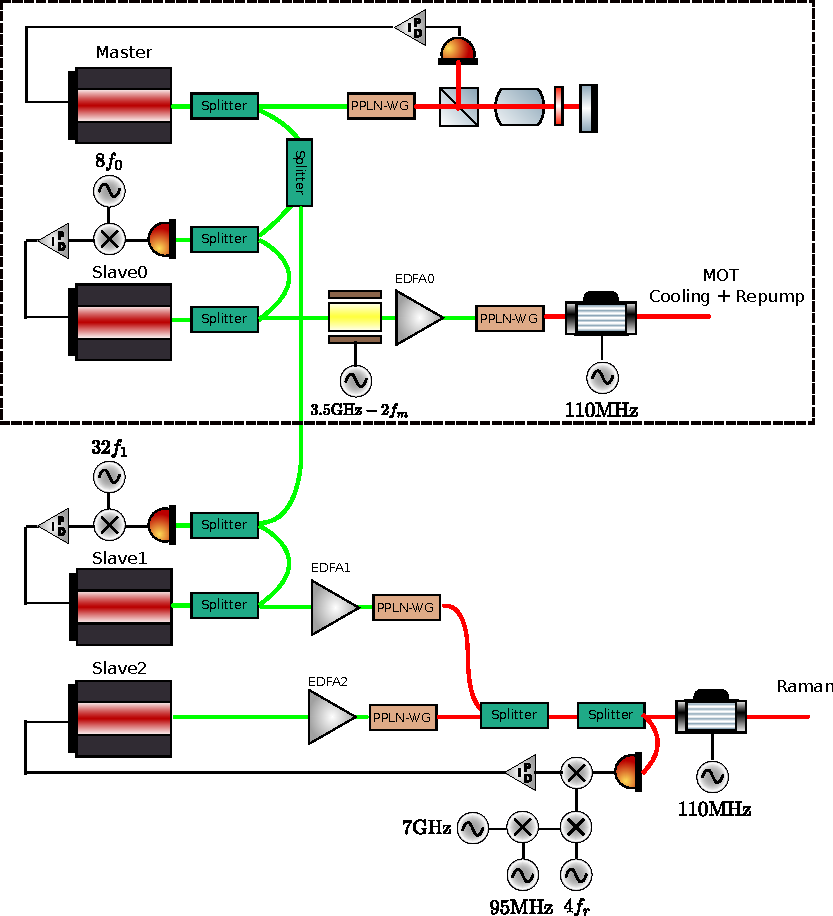
\includegraphics{muquans_schematic}
    \caption[\Muquans Laser System Diagram]{Schematic of the \Muquans laser system. Each output laser is derived from a 1560nm \acs{ecdl} (shown in green) which is amplified using an \acs{edfa} and then frequency-doubled to 780nm using a \acs{ppln} crystal. A master laser is locked to the 3,4 crossover in \ac{rb85} and the output lasers are offset-locked to their corresponding frequencies. The dashed region indicates the components used for generating light for the \acp{mots}, which was the only function of this laser for this experiment.}\label{fig:muquans_schematic}
\end{figure}
\subsection{Absolute Frequency Reference} \label{subsec:muquans_master}
The purpose of the master laser is to provide an absolute frequency reference so that the frequency of the output lasers can be controlled by comparing the difference frequency between them and the master. Lasers with linewidths narrower than their natural linewidth can be achieved by using a servo to stabilise their frequency and is essential for any experiment that requires laser light of a precise frequency. The frequency reference for the master is obtained using saturated absorption spectroscopy inside a Rubidium vapor cell. The sub-Doppler features in this spectrum are insensitive to temperature changes, and under sufficiently weak laser power have linewidths close to the natural linewidth of Rubidium (\(\Gamma \sim 2\pi \times 6\)MHz). \FigureRef{fig:muquans_satspec} shows the saturated absorption spectrum using the \Muquans master laser. This is obtained by fine adjustment of the temperature of the master \ac{ecdl}. The laser is set to lock to the crossover resonance between the \(F = 3 \rightarrow F' = 3\) and \(F = 3 \rightarrow F' =4 \) transitions in \ac{rb85} (indicated as \(b)\)), which is the strongest feature in the spectrum as well as being relatively close the the cooling transition in \ac{rb87} (indicated as \(a)\)).   
\begin{figure}
    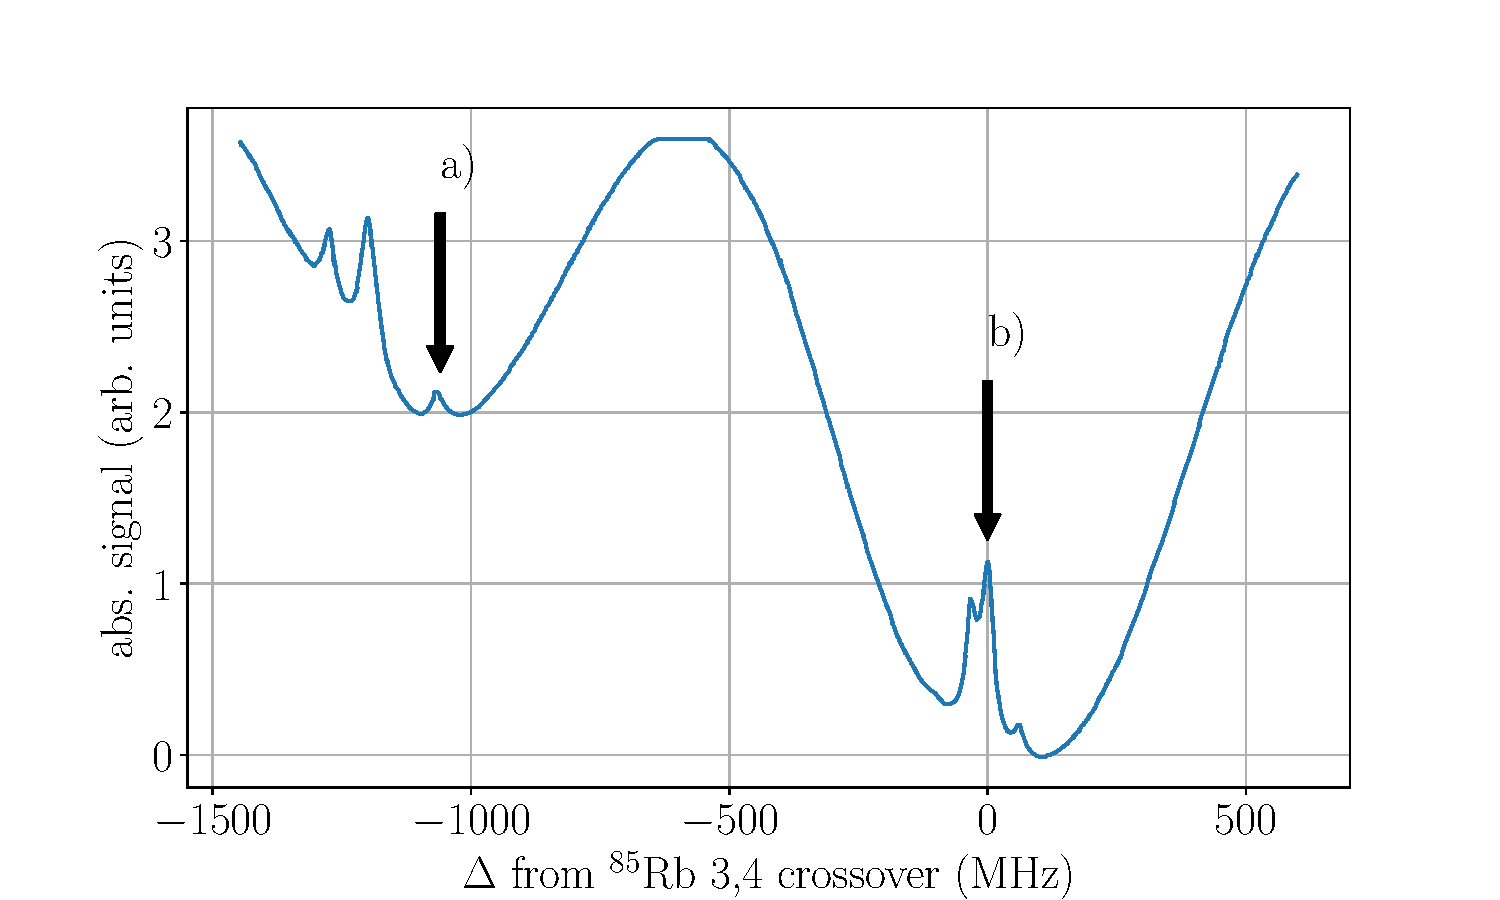
\includegraphics[width=0.6\textwidth]{sat_spec}
    \caption[Saturated absorption spectroscopy of the \Muquans master laser.]{Saturated absorption spectroscopy using the Rubidium vapour cell in the \Muquans laser. The absorption features indicated are \(a)\): the \(F = 2 \rightarrow F' = 3\) transition in \ac{rb87} and \(b)\): the crossover resonance between the \(F = 3 \rightarrow F' = 3\) and \(F = 3 \rightarrow F' =4 \) transitions in \ac{rb85} which is used to lock the frequency of the master laser.}
    \label{fig:muquans_satspec}
\end{figure}
\begin{figure}
    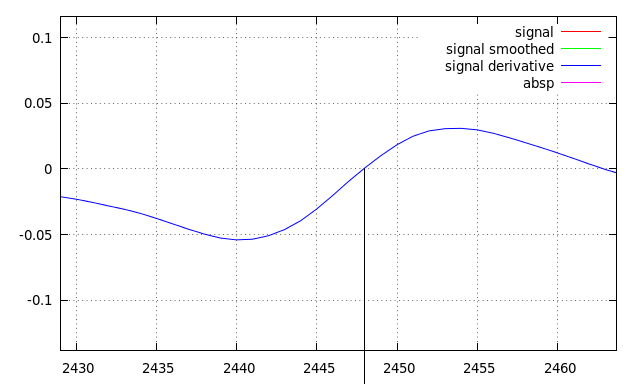
\includegraphics[width=0.6\textwidth]{error_signal}
    \caption[Error Signal for the \Muquans master servo.]{Error signal obtained by modulating the laser current. Close to the lock point, the signal is approximately linear. This signal is used in a feed-back loop to correct for frequency changes of the master laser.}
    \label{fig:muquans:error_signal}
\end{figure}
Some form of feed-back onto the master laser is required to keep its frequency fixed. The simplest way to achieve this is to use a signal that is linearly proportional to the deviation in frequency from the set-point, if one exists. The frequency of the laser is modulated by weakly modulating the current to the master \ac{ecdl}. {\textbf add more detail about the error signal lineshape} The error signal shown in \FigureRef{fig:muquans_errorsignal} is obtained by demodulating the absorption signal using a lock-in amplifier. In fact, this current modulation is always present on the master laser and the saturated absorption spectrum shown previously has been processed to average out the effects from this fast frequency modulation. In addition to proportional feed-back from the error signal, the servo that controls the master frequency also contains an integrator to compensate for long-term drifts. Typically, these arise from external temperature changes and if unaccounted for, they could cause the laser to unlock. In the conditions of our laboratory, where the temperature is externally controlled, this has never occurred.  
\subsection{Generating MOT light}
\subsection{Raman light}
\subsection{Real-time Frequency Control}
\section{The M-Squared Laser System}\label{sec:setup_msquared}
\verysubsection{To-Do}
\begin{itemize}
    \item Schematic
    \item Raman PLL phase-noise
    \item Laser Control
    \item DCS module
\end{itemize}
\subsection{Laser Specifications}
\subsection{The DCS Control Module}
\subsection{Frequency Control of the Raman Lasers}
\subsection{Controlling the Phase Difference}

    \chapter{MOTMaster}\label{chap:compinterface}

\section{Chapter Overview}\label{sec:compinterface_overview}
The aim of this chapter is to provide a description of the MOTMaster
software, which was developed from a pre-existing version during my PhD. The
design of MOTMaster assumes very little about the particular experiment it is
being used for, so much of the discussion in this chapter will be kept
general. This chapter begins with a motivating the need to extend MOTMaster by
developing a graphical interface to simplify the creation of experimental
sequences, as well as implementing new methods of controlling hardware. This
is followed by a description of how input and output channels are controlled using MOTMaster in~\SectionRef{sec:mm_interface}. The structure of a MOTMaster sequence, along with how it runs an experiment is then presented in~\SectionRef{sec:mm_sequences}. Finally, the specific hardware used in this experiment and an overview of each major step of the experiment is given in~\SectionRef{sec:mm_control_hardware}.

\section{Motivation}\label{sec:mm_motivation}
In the initial stages of my PhD, I decided to use Cicero Word
Generator~\cite{Keshet2012} to control the hardware for the experiment. This
is a graphical-based control system developed by Wolfgang Ketterle's group at
MIT, which was designed for controlling atomic physics experiments using
National Instruments hardware. Over time, as the experiment became more
complex, it started to become apparent that Cicero was not suited to meet all
of our requirements for control software. This was most evident in the
control of the M-Squared Raman laser system. Cicero also takes an
appreciable amount of time (around \sivalue{300}{\milli\second}) to
re-calculate the experiment sequence between each shot. Since the design of
Cicero was aimed at controlling experiments that take many seconds per cycle,
this dead time between each cycle is not significant on those time scales. In
contrast, each cycle of this experiment takes around
\sivalue{250}{\milli\second}. This unnecessary dead time needed to be
addressed if we hoped to improve the repetition rate. \par\noindent
After it became clear that a potentially large amount of work would be needed
to improve Cicero, I decided that it was worth moving to a new control
system. A collection of programs, named EDMSuite, has been developed by
people in \ac{ccm} to control a range of experiments within the group. One
application, MOTMaster, was designed to control and acquire data from
experiments investigating cold atoms trapped in a \ac{mot}. However, its method of structuring experimental sequences was
inconvenient, as it lacked an intuitive graphical user interface. During the
process of switching to using MOTMaster to control the experiment, I designed
a graphical method of structuring sequences, which functioned identically on
a device level to the original method of defining sequences. In addition to
this, I included an interface to the M Squared laser system, so that it could
be controlled using MOTMaster. A schematic of the structure of MOTMaster and how it interfaces with hardware is shown in~\FigureRef{fig:motmaster_structre}. It is designed so that experiments can be controlled without requiring specific details about the hardware in use.
\begin{figure}
    \centering
    \fontsize{16pt}{16pt}
    \resizebox{0.4\textwidth}{!}{\input{motmaster_structure.pdf_tex}}
    \caption[Schematic diagram of MOTMaster and hardware interface.]{Schematic diagram of MOTMaster and the hardware it controls. A sequence is built using the user interface, which then uses separate modules to communicate to the hardware. In this way, an experiment can be controlled without requiring specific knowledge of the hardware.}
    \label{fig:motmaster_structure}
\end{figure}
\section{Interfacing wth Hardware}\label{sec:mm_interface}

The majority of the experimental hardware is controlled using analogue and
digital voltages that are generated by \ac{daq} cards manufactured by
National Instruments. MOTMaster is compatible with cards that use either the
NI-DAQmx or NI-HSDIO device drivers. These are used to configure the
generation or acquisition of digital or analogue voltage waveforms. By design, they are
capable of precisely timing and synchronising their I/O across multiple
devices. Most components in the experiment rely on this precise timing to
function correctly. Other devices, where timing accuracy is less critical,
are controlled by sending or receiving data using serial communication. This
has the advantage of allowing more structured command beyond analogue or
digital voltages, but the communication speed of the serial channel limits
the accuracy of the execution time. \par\noindent
The following section describes the low-level interface between MOTMaster and the experimental hardware. It begins by introducing the concept of hardware abstraction in~\SectionRef{subsec:compinterface_hwabstraction}. This is followed by a more detailed discussion of how each type of control is implemented. \SectionRef{subsec:compinterface_patterngen} describes how analogue and digital output waveforms are generated. \SectionRef{subsec:compinterface_serial} outlines serial communication, along with a method for triggering this communication during an experiment. Finally, this section concludes with a discussion on acquiring analogue input data, which is given in~\SectionRef{subsec:compinterface_mmacquisition}.

\subsection{Hardware Abstraction}\label{subsec:compinterface_hwabstraction}
When designing software, it is often useful to structure a program in such a
way that modules which make use of other components do not need to know about
their specific implementation in order to use them. This approach means that the submodule can be modified without harming the
compatibility of these two components. In the context of experimental
hardware, this is equivalent to requiring that changing specific components,
for example the \ac{vco} that generates the RF power for an \ac{aom}, will
not stop the experiment from working. This is done using abstract
representations of the hardware, in the form of input and output channels
that are used to communicate to each device. 
\subsection{Voltage Pattern Generation}\label{subsec:compinterface_patterngen}
\subsubsection{Analogue Outputs}
All the analogue outputs controlled using MOTMaster are done using the
NI-DAQmx software. Each output uses a \ac{dac} to convert a floating-point
number into an analogue voltage. To generate a sequence of voltages across
multiple channels, the NI-DAQmx driver allocates a block of memory on the
\ac{daq} card for each output channel. This memory acts as a first-in
first-out (FIFO) buffer for data streamed to it from a computer. The output
of each channel is synchronised to a clock signal, so that every time a
rising edge occurs on the clock, the voltage at each output transitions to
the value corresponding to the next value in its corresponding buffer.
Channels across multiple \ac{daq} cards can be synchronised by sharing a
clock signal, which can be done using the bus that connects cards in a PXI-e
chassis. Additional cards can also be configured to trigger the start of
their output at the moment they receive the first clock pulse, rather than
waiting for a software trigger from the computer. \par\noindent
\subsubsection{Digital Outputs} 
Digital outputs from NI-DAQmx cards are generated in much the same way as
analogue voltages, except for the fact that they only take two values
corresponding to either a low (\sivalue{0}{\volt}) or high
(\sivalue{3.3/5}{\volt}) level. Additionally, \ac{daq} cards which use the
NI-HSDIO driver can be used. These cards can be sampled at much higher rates than NI-DAQmx ones. For instance, the NI-HSDIO PXI-6541 card can generate
digital voltages at sample rates up to \sivalue{50}{\mega\hertz}. Rather than writing the pattern as an array of
values at each clock cycle, the sequence is segmented into smaller patterns
during which the state of each channel is constant, as illustrated in
\FigureRef{fig:hsdio_timing}. NI-HSDIO cards can be scripted to generate each
of these patterns for the appropriate number of clock cycles.
\begin{figure}
    \centering
    \begin{tikztimingtable}
    Clock 20 MHz &[C] 50{0.5C} G \\
Channel 1 & 1L N(A1) 2L 1H N(A2) 1H N(A3) 4H N(A4) 6H 1L N(A5) 8L N(A6) 1L \\
Channel 2 & 4L 4H 15L 2H \\

\multirow{2}{*}{Waveform} & 1L ;[dotted]2L; 1H 1H ;[dotted]3H; 1H ;[dotted]6H; 1L ;[dotted]7L; 1L ;[dotted] 1L;\\
& 1L N(B1) ;[dotted]2L; 1L N(B2) 1H N(B3) ;[dotted]3H; 1L N(B4) ;[dotted]6L; 1L N(B5) ;[dotted]7L; 1H N(B6) ;[dotted] 1H;\\
\extracode
\tablerules
\begin{pgfonlayer}{background}
\foreach \n in {1,...,6}
\draw [help lines] (A\n) -- (B\n);
\end{pgfonlayer}
\end{tikztimingtable}

    \caption[Scripted pattern generation for an NI-HSDIO card]{Scripted
    pattern generation for an NI-HSDIO digital output card. A pattern is
    split into segments which correspond to a duration for which all the
    channels output a constant value. Each of these smaller waveforms are
    written to the on-board memory, along with a script that instructs the
    card to output each pattern for the required number of times to
    reconstruct the original sequence. By reducing the amount of memory
    required to define the sequence, a faster clock frequency and hence
    timing resolution can be used to output digital control
    signals.}\label{fig:hsdio_timing}
\end{figure}
\subsection{Timed Serial Communication}\label{subsec:compinterface_serial}
Serial communication is used to control devices which require more complex
control than is possible using analogue or digital voltages. This increase in
complexity comes at the cost of slower response times, because it takes
longer to communicate an array of bytes than to change the voltage
across an output terminal. Using the NI-VISA driver, the output of serial
data can only be timed using a software clock on a computer, which is more
prone to jitter than a hardware clock. One way to improve the synchronisation
between serial data and hardware timed outputs is to use extra hardware to
trigger the transmission of serial data. If the trigger is timed using the
same clock as other outputs and the transmission delay is accounted for, then
serial data can be output more synchronously. The scheme for timing serial
messages is shown in \FigureRef{fig:serial_timing}. Serial messages are
stored as strings on the computer and a counter channel is configured so that
every time it detects a rising edge, the computer outputs the next message.
This counter is connected to a digital output channel, so that it acts as a
trigger for the serial data output. Using this method, multiple serial
messages can be sent to one device during a sequence even for devices which
have no means of storing commands.
\begin{figure}
    \centering
    
\begin{tikztimingtable}
    Trigger & 2L 1H 6L 1H 3L\\
    Counter & 2D{0}7D{1}3D{2}\\
    Serial & 4.7z3.5D{M0}6.8z2D{M1}1Z\\
    \extracode
    \tablerules
    
    \end{tikztimingtable}
    \caption[Timing diagram for serial communication]{Timing diagram for
    serial communication. A counter channel is configured to count edges from
    a digital output channel. Every time it sees a rising edge, it triggers
    the output of the next message on each serial channel from the computer.
    Multiple messages can be communicated during a single sequence without
    the need for software timing.}\label{fig:serial_timing}
\end{figure} 
\subsection{Voltage Acquisition}\label{subsec:compinterface_mmacquisition}
Analogue input channels are configured in a similar way to analogue output
channels. A block of memory is allocated on the \ac{daq} card for each input
channel. Once the card is triggered to start acquiring, an \ac{adc} converts
the voltage across the input into a digital value at every rising edge of the
clock signal. Once the sequence has finished, or the buffer has been filled,
the card streams this data to the computer.

\section{MOTMaster Sequences}\label{sec:mm_sequences}
In addition to interfacing with control hardware, MOTMaster is used to define
the structure of experimental sequences. In earlier versions of MOTMaster,
sequences were defined using functions within a C\# source file. To run an
experiment, MOTMaster compiled this file to build the voltage patterns and
wrote them to the hardware. Whilst this had little overhead in resources
needed to build and run a sequence, modifying and debugging sequences was
much more time consuming. Taking inspiration from Cicero, the user interace
of MOTMaster was redesigned so that sequences could be expressed graphically.
They are then built using the same functions as before, so that from the
point of view of the hardware, the two methods of control are equivalent. 

\subsection{Sequence Structure}
A MOTMaster sequence is composed of a list of sequence steps, which define
the state of the control hardware over a discrete amount of time. Each step
contains the following properties:
\begin{itemize}
    \item \underline{Name}: A descriptive name for the step.
    \item \underline{Duration}: duration of the step, which must be an integer multiple of the timebase (e.g. \sivalue{10}{\micro\second} for a \sivalue{100}{\kilo\hertz}
    sample clock frequency).
    \item \underline{Serial Channel}: A serial message encoded as a string of text.
    \item \underline{Digital Output Channel}: High (\sivalue{3.3}{\volt}) or Low (\sivalue{0}{\volt})
    \item \underline{Analogue Output Channel}: Single value, step or ramp the output from a start to end value, or output an arithmetic function over time.
\end{itemize}
where each individual output channel has its own property.
\par\noindent
A sequence step is useful to represent a single action, so that each
stage of the experiment, for example the initial \ac{mot} loading phase, is
composed of multiple steps. Numerical values, such as analogue voltages or
times, can be represented by named parameters. The value of a parameter can
be updated between each cycle of the experiment, so that MOTMaster can
implement a scan by iterating a parameter through a range of values. The sequence steps are also used to
define when to acquire from the analogue inputs. A specific digital channel,
named \verb|acquisitionTrigger|, is reserved as a start trigger for the
acquisition. This channel is also used to define the length of time over which to acquire data. Analogue data acquisition is triggered at the start of the step where this channel goes high and stops when it goes low. 
\subsection{Running a Sequence}
MOTMaster is designed to run in two modes, referred to as repeat and scan.
The distinction between these is that the repeat mode does not need to
recreate a sequence between each cycle. Before MOTMaster starts controlling
the experiment, the sequence is built once and the output hardware is configured
to regenerate their patterns. This reduces the delay between
each cycle, which is largely a result of the time needed to process acquired
data and reconfigure the control hardware. In contrast, scan mode varies a
parameter during each cycle, so additional time is required to rebuild the
sequence and write to each \ac{daq} card. Aside from this, these modes
operate equivalently. \par\noindent
At the start of an experiment cycle, the hardware is
initialised and timing properties, such as the trigger and sample clock for
each \ac{daq} card is set. An example of a sequence as repreented in the user interface is shown in~\FigureRef{fig:motmaster_sequence}. This is
converted into the analogue and digital voltage patterns for each \ac{daq}
card. The required buffer for the analogue input
data is calculated based on the state of the \verb|acquisitionTrigger|
channel. If any serial commands are used, the timing properties of the
counter channel are configured, similarly to the rest of the \ac{DAQ}
hardware. The sequence is started by sending a software trigger to one output
card, which is configured to export its start trigger to the other cards.
This ensures that start of the output of each card is synchronised. 
\begin{figure}
    \centering
    \resizebox{0.5\textwidth}{!}{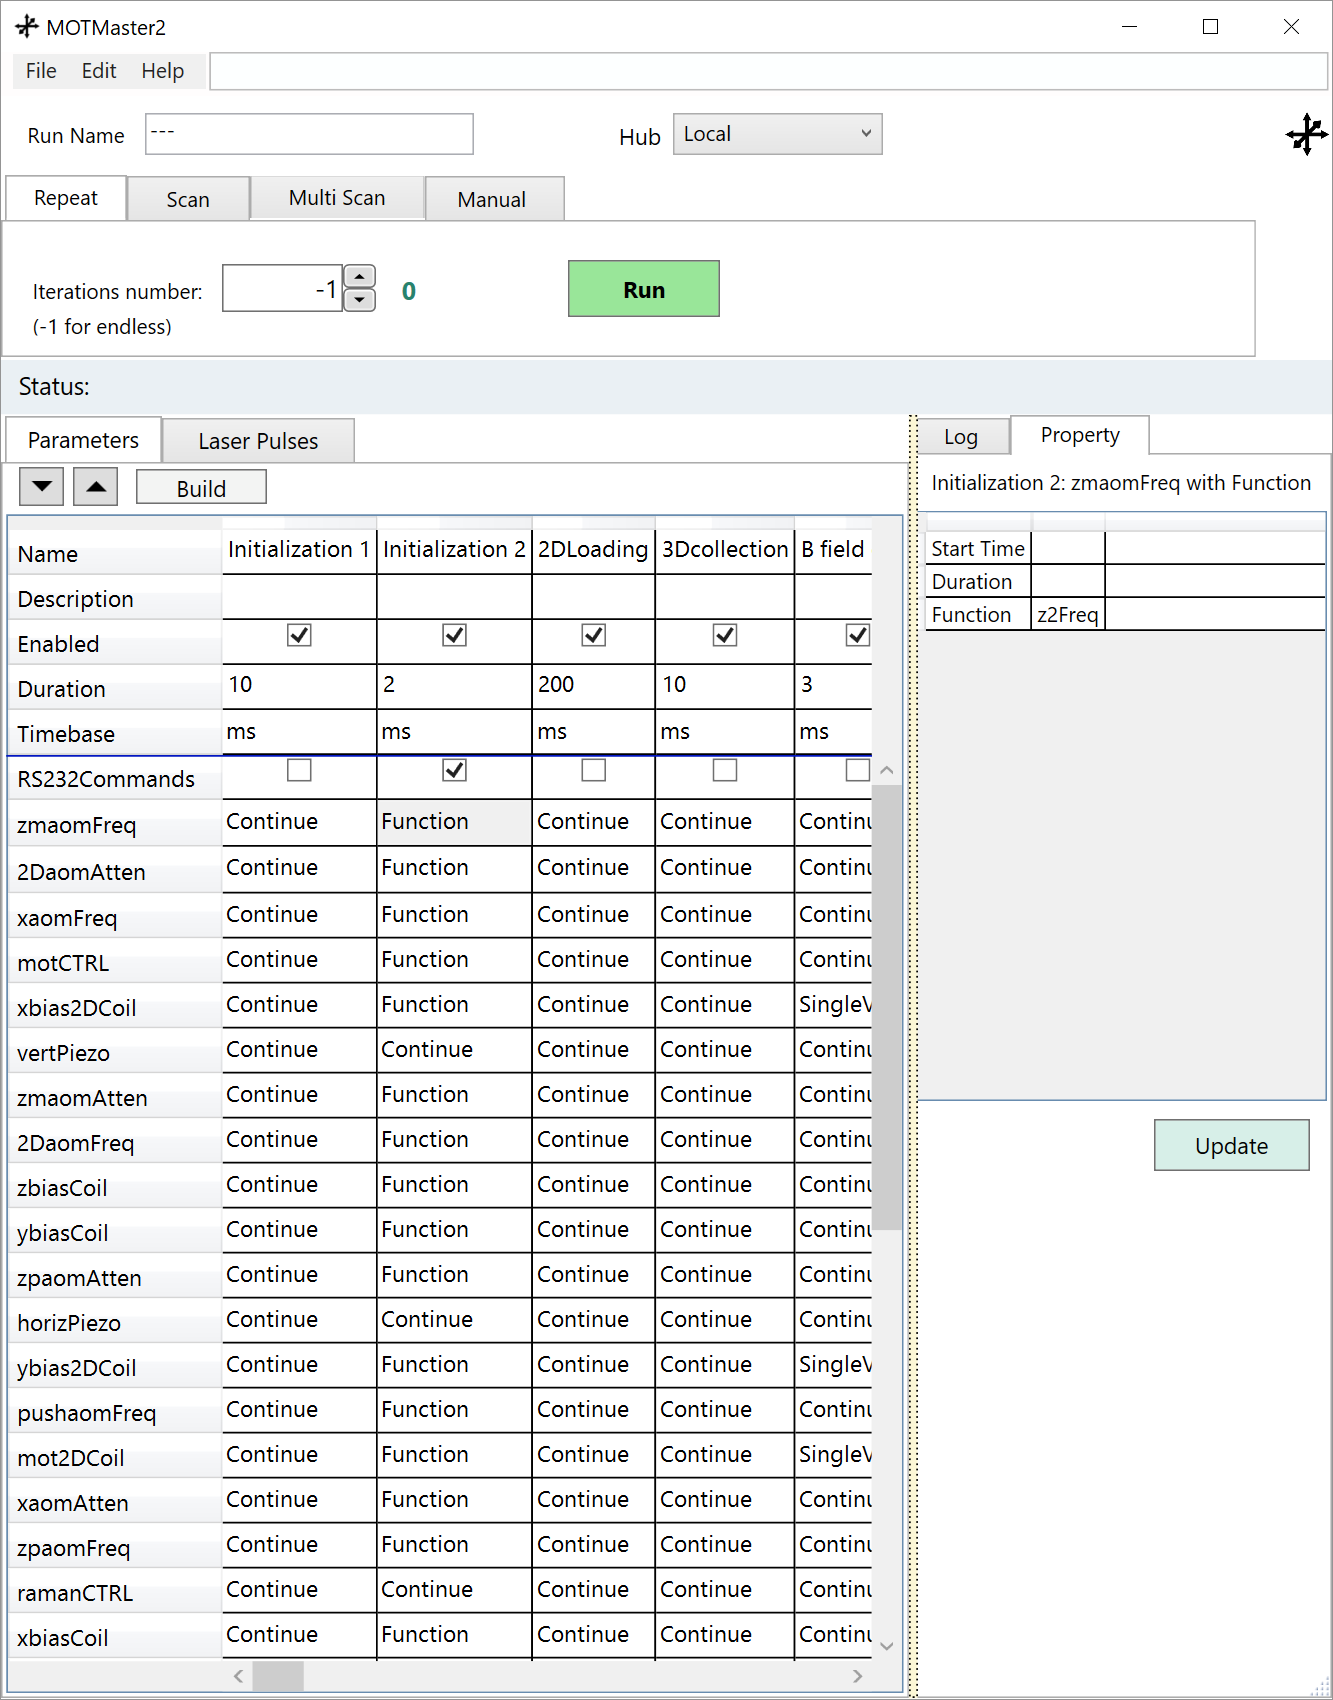
\includegraphics{motmaster_sequence.png}}
    \caption[MOTMaster user interface]{A sequence as represented in the MOTMaster user interface. Each step defines a duration and properties for each output channel. The sequence can either be run repeatedly, or configured to iterate through values of a chosen parameter.}
    \label{fig:motmaster_sequence}
\end{figure}
\par\noindent
After the sequence has finished, any acquired data from the analogue input channels is
streamed to the computer. The data per channel are segmented into arrays that
were acquired during each sequence step, before additional post-processing if
required. Finally, the hardware is reset to its initial state, before
starting the next experiment cycle.

\section{Experiment Control Hardware}\label{sec:mm_control_hardware}
In the preceding sections, the discussion of MOTMaster has been presented
without referring to specific hardware used in this experiment. Subsequent
chapters will introduce components of the experiment that are controlled by a
computer, but it is worth introducing the hardware used to implement this
control. A diagram of the control hardware is shown in~\FigureRef{fig:control_hardware}. All of the \ac{daq} cards are housed on a PXIe-1073 chassis, so that
timing signals such as start triggers and sample clocks can be shared on the
PXI backplane. The analogue output signals are generated on a
PXI-6723 card. This contains 32 analogue output channels and the output of
each is generated using a 13 bit \ac{dac}. Over the maximum voltage range of
\(\pm \sivalue{10}{\volt}\), this corresponds to an output quantisation of
\sivalue{2.44}{\milli\volt}, which did not limit the precision of any
analogue control in the experiment. The analogue output pattern is sampled at
a frequency of \sivalue{100}{\kilo\hertz}, which gives a minimum resolution
of \sivalue{10}{\micro\second}. Any jitter on this sample clock did not
produce any noticeable effects during the experiment. \par\noindent
Two cards on the chassis are able to acquire data from analogue inputs. The
first is a PXIe-6341, which has 16 input channels, each with a 16-bit
\ac{adc}. In addition to this, a counter channel on this card was used to trigger the output of serial messages. During the preliminary stages of the experiment, this bit-depth was
sufficiently large to prevent quantisation effects becoming significant. However
the AI-Q-2010 MEMS accelerometer used in the experiment, discussed further in \SectionRef{subsec:raman_mems}, has an equivalent voltage noise below this quantisation level. Therefore, a
PXI-4462 card, which contains 4 24-bit analogue input channels, was added.
This card is used to acquire data from devices where the higher voltage
resolution is desirable --- namely, the MEMS accelerometer and the
photodiode used to detect the population of atoms in each state after interference.\par\noindent
Digital output signals are generated using a PXI-6541 card. Unlike the
others, this card is controlled using the NI-HSDIO driver. With a maximum
sampling frequency of \sivalue{50}{\mega\hertz}, this card is capable of
generating digital signals at a much higher rate than the PXIe-6341, which
also contains digital output channels. However, the PXIe-6341 card only
contains 8 digital channels that can be timed using a hardware clock, fewer
than required to control the entire experiment.
\par\noindent
Two components of the experiment are controlled during the experiment using
serial communication. The first of these is an interface to the \ac{dds} on
the \Muquans\ laser which control the frequency of the cooling and repump
lasers and is controlled in real-time during the experiment. This
communication protocol is described in further detail in
\SectionRef{subsec:muquans_comm}. Finally, MOTMaster is configured to remotely connect to the M
Squared laser, so that it can control all the parameters necessary to drive
Raman transitions during the experiment. This is done by sending structured
JSON messages that contain commands to implement this control. More detail on how this is used in the experiment is given in
\SectionRef{subsuc:msquared_comm}.
\begin{figure}
    \centering
    \fontsize{16pt}{14pt}
    \resizebox{1\textwidth}{!}{\input{control_hardware.pdf_tex}}
    \caption[Control hardware schematic diagram]{Schematic diagram of the control hardware. The PXIe chassis contains the DAQ cards which generate the analogue and digital waveforms used to control other devices. Signals are routed between the cards to synchronise their operation. Serial communication to the \Muquans laser (\SectionRef{sec:muquans_light}), the M-Squared laser (\SectionRef{sec:msquared_laser})and the CCD camera (\SectionRef{sec:imaging}) are used for their control.}
    \label{fig:control_hardware}
\end{figure}

\section{Experimental Sequence Overview}
The experiment can be broken down into the following stages:
\begin{itemize}
    \item \underline{Loading}: Atoms are loaded from the 2D \ac{mot} into the 3D \ac{mot}.
    \item \underline{Molasses}: Atoms are released from the trap and cooled further in an optical molasses.
    \item \underline{State Preparation}: A sequence of optical and microwave pulses are used to prepare atoms with a narrow velocity spread in the \(\ket{1,0}\) state.
    \item \underline{Interferometry}: A \(\pi/2 - \pi - \pi/2\) sequence of laser pulses drive Raman transitions between the atoms.
    \item \underline{Dectection}: Two laser pulses are used to measure the number of atoms in \(\ket{F=2}\) and the total number, respectively. From these measurements, the interferometer phase difference can be inferred.
\end{itemize}

\end{mainmatter}

\begin{appendices}
    \chapter*{Acronyms}
    \begin{acronym}
        \acro{ccm}[CCM]{Centre for Cold Matter}
        \acro{rb87}[\(^{87}\)Rb]{Rubidium-87}
        \acro{rb85}[\(^{85}\)Rb]{Rubidium-85}
        \acro{mot}[MOT]{Magneto-optical Trap}
        \acro{aom}[AOM]{Acousto-optic Modulator}
        \acro{eom}[EOM]{Electro-optic Modulator}
        \acro{pm}[PM]{Polarisation-Maintaining}
        \acro{qwp}[QWP]{Quarter-wave Plate}
        \acro{hwp}[HWP]{Half-wave Plate}
        \acro{mfd}[MFD]{Mode Field Diameter}
        \acro{ppln}[PPLN]{Periodically Poled Lithium Niobate}
        \acro{pll}[PLL]{Phase-Locked Loop}
        \acro{fpga}[FPGA]{Field-Programmable Gate Array}
        \acro{edfa}[EDFA]{Erbium-Doped Fibre Amplifier}
        \acro{ecdl}[ECDL]{External-Cavity Diode Laser}
        \acro{ttl}[TTL]{Transistor-transistor Logic Circuit}
        \acro{ni}[NI]{National Instruments}
        \acro{daq}[DAQ]{Data Acquisition}
        \acro{vco}[VCO]{Voltage-Controlled Oscillator}
        \acro{adc}[ADC]{Analogue-to-Digital Converter}
        \acro{dac}[DAC]{Digital-to-Analogue Converter}
        \acro{hal}[HAL]{Hardware Abstraction Layer}
        \acro{spi}[SPI]{Serial Programming Interface}
        \acro{dds}[DDS]{Direct Digital Synthesiser}
        \acrodefplural{aom}[AOMs]{Acousto-optic Modulators}
        \acrodefplural{ecdl}[ECDLs]{External-Cavity Diode Lasers}
        \acrodefplural{edfa}[EDFAs]{Erbium-Doped Fibre Amplifiers}
        \acrodefplural{ttl}[TTLs]{Transistor-transistor Logic Circuits}
        \acrodefplural{mots}[MOTs]{Magneto-optical Traps}
        \acro{pbs}[PBS]{Polarising beam-splitter}
        \acro{dro}[DRO]{Dielectric Resonator Oscillator}
    \end{acronym}


\chapter{Laser Systems}\label{chap:setup}
This chapter provides a description of the hardware that makes up the experiment. Over the course of the project, the complexity of the experiment necessarily increased. The setup is presented in a bottom-up approach, starting from the most fundamental components, to provide a clear overview of the system. \\

\verysubsection{To-Do}
\begin{itemize}\item Figures describing each of the lasers
    \item Describe 3D and 2D MOT setups  
    \item Imaging systems
    \item Microwave synthesisers
    \item Raman Assembly
    \item MOT light distribution
\end{itemize}
\section{Chapter Overview}\label{sec:setup_overview}
The first two sections describe the two commercial laser systems used in this experiment. The \Muquans\ laser system which generates the light used for cooling and repump in the 2D and 3D \acp{mots}, referred to as the \acs{mot} light. The design and operation of this laser is given in \SectionRef{sec:setup_muquans}. A secondary laser system, built by MSquared, is used to generate light to drive Raman transitions between two hyperfine ground states in \ac{rb87}\footnote{The \Muquans\ laser also has a pair of lasers designed for driving Raman transitions, but these are not used in this experiment. \SectionRef{sec:setup_msquared} gives an explanation for this.}, otherwise referred to as Raman light. This is described in \SectionRef{sec:setup_msquared}.This is followed by a description of the vacuum chamber in \SectionRef{sec:setup_chamber} which contains both the 2D \ac{mot} (\SectionRef{subsec:setup_2DMOT}) and the 3D \ac{mot} (\SectionRef{subsec:setup_3DMOT}).  

\section{The \Muquans\ Laser System}\label{sec:setup_muquans}
\verysubsection{To-Do}
\begin{itemize}
    \item Laser Schematic
    \item Plots of lock signals
    \item DDS Serial communication
    \item Power output, stability
    \item Ref for error signal generation by current modulation
    \item Move some of this to appendix
\end{itemize}
All the \ac{mot} light in this experiment was generated by the \Muquans\ laser~\cite{muquansWebPage}. \Muquans\ is a French laser company that is a spin-off from the Institut d'Optique and Observatoire de Paris. Consequently, their technology has been developed over a long history of performing experiments into atom interferometry using Rubidium. A schematic of this laser system is shown in \FigureRef{fig:muquans_schematic}. The \Muquans\ laser is comprised of four 1560nm \acp{ecdls} which are frequency-doubled to produce light at wavelengths close to 780nm. The telecommunications industry, which relies heavily on light in the 1530--1565nm wavelength band for optical communications, has motivated a rapid development in low-noise, robust lasers. In particular, this has enabled a design which does not require free-space optics and is much more resilient to effects such as temperature changes and vibrations, when compared to more conventional 780nm laser systems. The \Muquans\ laser contains one master laser\footnote{see \SectionRef{subsec:muquans_master} for more details}, which is locked to the \(F = 3 \rightarrow F' = 3,4\) crossover point in \ac{rb85}, and serves as an absolute frequency reference. The other three slave lasers are used for output. The first one is used to provide light for cooling, as well as repump light by modulating the phase of this laser using an \ac{eom}. The other two make up a pair of lasers for driving Raman transitions. One laser is frequency-offset locked to the master and the other is phase-locked to the first, to ensure that the relative phase between the two lasers is constant. It should be noted that this Raman laser was not used in this experiment, so will not be discussed in great detail. Each of these slave lasers is amplified in an \ac{edfa} before being frequency doubled in a \ac{ppln} and passed through an \ac{aom} which is used to control the output power during the experiment.
\begin{figure}
    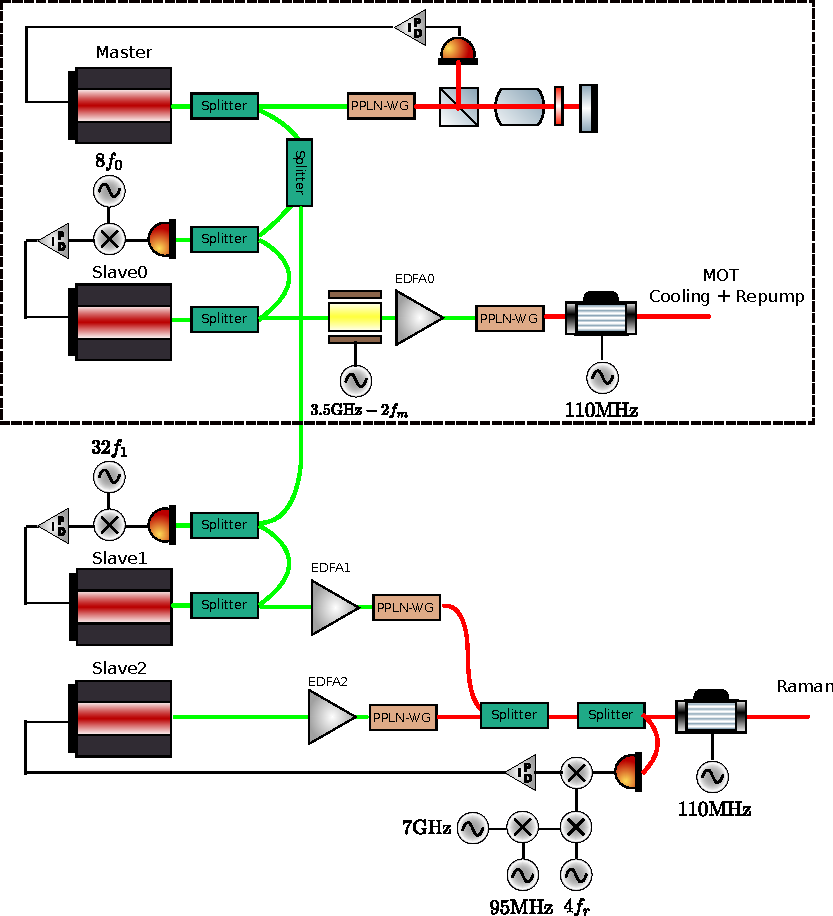
\includegraphics{muquans_schematic}
    \caption[\Muquans\ Laser System Diagram]{Schematic of the \Muquans\ laser system. Each output laser is derived from a 1560nm \acs{ecdl} (shown in green) which is amplified using an \acs{edfa} and then frequency-doubled to 780nm using a \acs{ppln} crystal. A master laser is locked to the 3,4 crossover in \ac{rb85} and the output lasers are offset-locked to their corresponding frequencies. The dashed region indicates the components used for generating light for the \acp{mots}, which was the only function of this laser for this experiment.}\label{fig:muquans_schematic}
\end{figure}
\subsection{Absolute Frequency Reference}\label{subsec:muquans_master}
The purpose of the master laser is to provide an absolute frequency reference so that the frequency of the output lasers can be controlled by comparing the difference frequency between them and the master. Lasers with linewidths narrower than their natural linewidth can be achieved by using a servo to stabilise their frequency and is essential for any experiment that requires laser light of a precise frequency. The frequency reference for the master is obtained using saturated absorption spectroscopy inside a Rubidium vapour cell. The sub-Doppler features in this spectrum are insensitive to temperature changes, and under sufficiently weak laser power have linewidths close to the natural linewidth of Rubidium (\(\Gamma \sim 2\pi \times 6\)MHz). \FigureRef{fig:muquans_satspec} shows the saturated absorption spectrum using the \\Muquans\ master laser. This is obtained by fine adjustment of the temperature of the master \ac{ecdl}. The laser is set to lock to the crossover resonance between the \(F = 3 \rightarrow F' = 3\) and \(F = 3 \rightarrow F' =4 \) transitions in \ac{rb85} (indicated as \(b\)), which is the strongest feature in the spectrum as well as being relatively close the the cooling transition in \ac{rb87} (indicated as \(a\)).   
\begin{figure}
    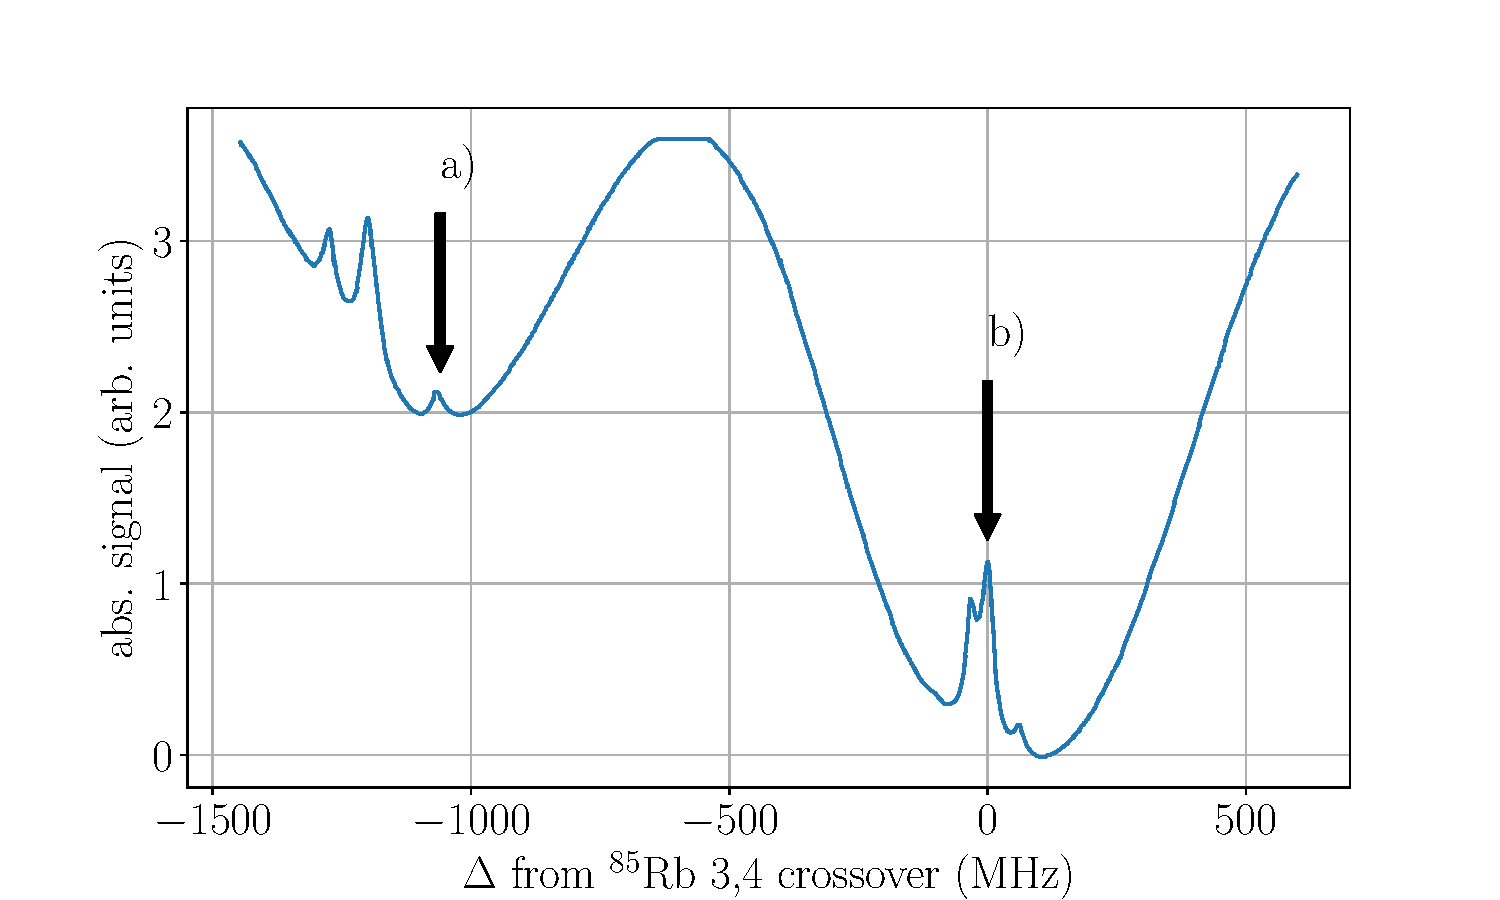
\includegraphics[width=0.6\textwidth]{sat_spec}
    \caption[Saturated absorption spectroscopy of the \\Muquans\ master laser.]{Saturated absorption spectroscopy using the Rubidium vapour cell in the \Muquans\ laser. The absorption features indicated are \(a\): the \(F = 2 \rightarrow F' = 3\) transition in \ac{rb87} and \(b\): the crossover resonance between the \(F = 3 \rightarrow F' = 3\) and \(F = 3 \rightarrow F' =4 \) transitions in \ac{rb85} which is used to lock the frequency of the master laser.}\label{fig:muquans_satspec}
\end{figure}
\begin{figure}
    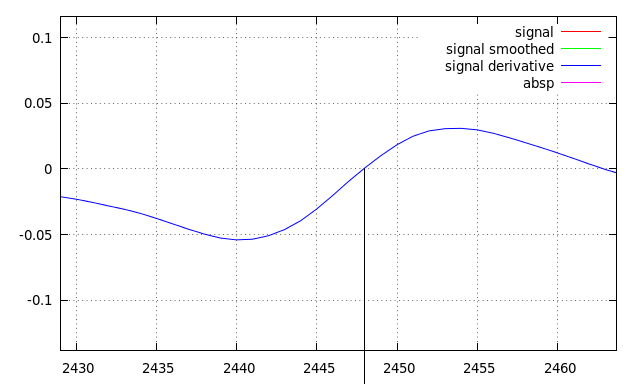
\includegraphics[width=0.6\textwidth]{error_signal}
    \caption[Error Signal for the \Muquans\ master servo.]{Error signal obtained by modulating the laser current. Close to the lock point, the signal is approximately linear. This signal is used in a feed-back loop to correct for frequency changes of the master laser.}\label{fig:muquans:error_signal}
\end{figure}
Some form of feed-back onto the master laser is required to keep its frequency fixed. The simplest way to achieve this is to use a signal that is linearly proportional to the deviation in frequency from the set-point, if one exists. The frequency of the laser is modulated by weakly modulating the current to the master \ac{ecdl}. {\textbf add more detail about the error signal lineshape} The error signal shown in \FigureRef{fig:muquans_errorsignal} is obtained by demodulating the absorption signal using a lock-in amplifier. In fact, this current modulation is always present on the master laser and the saturated absorption spectrum shown previously has been processed to average out the effects from this fast frequency modulation. In addition to proportional feed-back from the error signal, the servo that controls the master frequency also contains an integrator to compensate for long-term drifts. Typically, these arise from external temperature changes and if unaccounted for, they could cause the laser to unlock. In the conditions of our laboratory, where the temperature is externally controlled, this has never occurred.  
\subsection{Generating MOT light}
\subsection{Raman light}
\subsection{Real-time Frequency Control}
\section{The M-Squared Laser System}\label{sec:setup_msquared}
\verysubsection{To-Do}
\begin{itemize}
    \item Schematic
    \item Raman PLL phase-noise
    \item Laser Control
    \item DCS module
\end{itemize}
\subsection{Laser Specifications}
\subsection{The DCS Control Module}
\subsection{Frequency Control of the Raman Lasers}
\subsection{Controlling the Phase Difference}

\end{appendices}

\begin{backmatter}
    \bibliographystyle{lucas_unsrt}
\bibliography{Thesis}
%\printbibliography

\chapter*{Acronyms}
\addcontentsline{toc}{chapter}{Acronyms}
\markboth{ACRONYMS}{}
\begin{acronym}
        \acro{adc}[ADC]{Analogue-to-Digital Converter}
        \acro{aom}[AOM]{Acousto-optic Modulator}
        \acro{ccm}[CCM]{Centre for Cold Matter}
        \acro{dac}[DAC]{Digital-to-Analogue Converter}
        \acro{daq}[DAQ]{Data Acquisition}
        \acro{dro}[DRO]{Dielectric Resonator Oscillator}
        \acro{dds}[DDS]{Direct Digital Synthesiser}
        \acro{ecdl}[ECDL]{External-Cavity Diode Laser}
        \acro{edfa}[EDFA]{Erbium-Doped Fibre Amplifier}
        \acro{eom}[EOM]{Electro-optic Modulator}
        \acro{fpga}[FPGA]{Field-Programmable Gate Array}
        \acro{gnss}[GNSS]{Global Navigation Satellite System}
        \acro{hal}[HAL]{Hardware Abstraction Layer}
        \acro{hwp}[HWP]{Half-wave Plate}
        \acro{mfd}[MFD]{Mode Field Diameter}
        \acro{mot}[MOT]{Magneto-optical Trap}
        \acro{na}[NA]{Numerical Aperture}
        \acro{neg}[NEG]{Non-evaporative Getter}
        \acro{nep}[NEP]{noise-equivalent power}
        \acro{ni}[NI]{National Instruments}
        \acro{pbs}[PBS]{Polarising beam-splitter}
        \acro{pll}[PLL]{Phase-Locked Loop}
        \acro{pm}[PM]{Polarisation-Maintaining}
        \acro{ppln}[PPLN]{Periodically-Poled Lithium Niobate}
        \acro{qwp}[QWP]{Quarter-wave Plate}
        \acro{sdlc}[SDLC]{sub-Doppler laser cooling}
        \acro{spi}[SPI]{Serial Programming Interface}
        \acro{ttl}[TTL]{Transistor-transistor Logic Circuit}
        %\acro{rb85}[\(^{85}\)Rb]{Rubidium-85}
        \acro{uhv}[UHV]{Ultra-high Vacuum}
        \acro{vca}[VCA]{Voltage-Controlled Attenuator}
        \acro{vco}[VCO]{Voltage-Controlled Oscillator}
        \acro{vsr}[VSR]{Velocity-selective resonance}
        \acrodefplural{aom}[AOMs]{Acousto-optic Modulators}
        \acrodefplural{ecdl}[ECDLs]{External-Cavity Diode Lasers}
        \acrodefplural{edfa}[EDFAs]{Erbium-Doped Fibre Amplifiers}
        \acrodefplural{ttl}[TTLs]{Transistor-transistor Logic Circuits}
        \acrodefplural{mots}[MOTs]{Magneto-optical Traps}
        \acro{rb87}[\(^{87}\)Rb]{Rubidium-87}
    \end{acronym}

    \begin{acronym}
        \acro{adc}[ADC]{Analogue-to-Digital Converter}
        \acro{aom}[AOM]{Acousto-optic Modulator}
        \acro{ccm}[CCM]{Centre for Cold Matter}
        \acro{dac}[DAC]{Digital-to-Analogue Converter}
        \acro{daq}[DAQ]{Data Acquisition}
        \acro{dro}[DRO]{Dielectric Resonator Oscillator}
        \acro{dds}[DDS]{Direct Digital Synthesiser}
        \acro{ecdl}[ECDL]{External-Cavity Diode Laser}
        \acro{edfa}[EDFA]{Erbium-Doped Fibre Amplifier}
        \acro{eom}[EOM]{Electro-optic Modulator}
        \acro{fpga}[FPGA]{Field-Programmable Gate Array}
        \acro{gnss}[GNSS]{Global Navigation Satellite System}
        \acro{hal}[HAL]{Hardware Abstraction Layer}
        \acro{hwp}[HWP]{Half-wave Plate}
        \acro{mfd}[MFD]{Mode Field Diameter}
        \acro{mot}[MOT]{Magneto-optical Trap}
        \acro{na}[NA]{Numerical Aperture}
        \acro{neg}[NEG]{Non-evaporative Getter}
        \acro{nep}[NEP]{noise-equivalent power}
        \acro{ni}[NI]{National Instruments}
        \acro{pbs}[PBS]{Polarising beam-splitter}
        \acro{pll}[PLL]{Phase-Locked Loop}
        \acro{pm}[PM]{Polarisation-Maintaining}
        \acro{ppln}[PPLN]{Periodically-Poled Lithium Niobate}
        \acro{qwp}[QWP]{Quarter-wave Plate}
        \acro{sdlc}[SDLC]{sub-Doppler laser cooling}
        \acro{spi}[SPI]{Serial Programming Interface}
        \acro{ttl}[TTL]{Transistor-transistor Logic Circuit}
        %\acro{rb85}[\(^{85}\)Rb]{Rubidium-85}
        \acro{uhv}[UHV]{Ultra-high Vacuum}
        \acro{vca}[VCA]{Voltage-Controlled Attenuator}
        \acro{vco}[VCO]{Voltage-Controlled Oscillator}
        \acro{vsr}[VSR]{Velocity-selective resonance}
        \acrodefplural{aom}[AOMs]{Acousto-optic Modulators}
        \acrodefplural{ecdl}[ECDLs]{External-Cavity Diode Lasers}
        \acrodefplural{edfa}[EDFAs]{Erbium-Doped Fibre Amplifiers}
        \acrodefplural{ttl}[TTLs]{Transistor-transistor Logic Circuits}
        \acrodefplural{mots}[MOTs]{Magneto-optical Traps}
        \acro{rb87}[\(^{87}\)Rb]{Rubidium-87}
    \end{acronym}


\end{backmatter}

\end{document}